%\documentclass[prodmode,acmtecs]{acmconf} % Aptara syntax
\documentclass[10pt, conference, compsocconf]{IEEEtran}
\usepackage{url}
\usepackage{ulem}
\usepackage{graphicx}
\usepackage{amsmath}
\usepackage{color}
\usepackage[ruled]{algorithm2e}
\usepackage{multirow}

\newcommand{\sui}[1]{%
  \textcolor{green}{SC-#1}
}

\newcommand{\marc}[1]{%
  \textcolor{red}{[MC: #1]}
}

\newcommand{\greg}[1]{%
  \textcolor{blue}{GB: #1}
}

%\ConferenceShortName{ICS}
%\ConferenceName{International Conference on Supercomputing}

\title{Comprehensive Algorithmic Resilience for \\Numeric Applications}
%\author{Sui Chen,
%\affil{Louisiana State University}
%Greg Bronevetsky,
%\affil{Lawrence Livermore National Laboratory}
%Marc Casas,
%\affil{Barcelona Supercomputing Center}
%Lu Peng
%\affil{Louisiana State University}}

\author{\IEEEauthorblockN{Sui Chen}
\IEEEauthorblockA{Louisiana State \\ University}
\and
\IEEEauthorblockN{Greg Bronevetsky}
\IEEEauthorblockA{Lawrence Livermore \\ National Laboratory}
\and
\IEEEauthorblockN{Marc Casas-Guix}
\IEEEauthorblockA{Barcelona Supercomputing \\ Center}
\and
\IEEEauthorblockN{Lu Peng}
\IEEEauthorblockA{Louisiana State \\ University}
}

\begin{document}

\maketitle
\begin{abstract}

As High-Performance Computing (HPC) systems become larger and more complex and their circuit feature sizes shrink, the systems become increasingly vulnerable to soft faults.
Since such faults may cause application crashes or may silently corrupt application results it is necessary to develop techniques to protect applications from such errors at a low cost in performance and power.
Since general-purpose resilience mechanisms, such as replication, can be very expensive it is imperative to develop ways to tailor resilience techniques to each application's properties and the needs of its users.

Extensive ongoing work on algorithmic techniques to detect and tolerate errors in common scientific sub-routines and kernels has proven their effectiveness.
However, their practical utility has been limited by the fact that real scientific applications (i) are significantly more complex than these simple kernels and (i) are vulnerable to a wider range of errors than most algorithmic checkers focus on.
To make scientific applications resilient to soft errors it is necessary to comprehensively combine resilience techniques that tolerate \emph{all} the major types of application errors.
Further, each technique must be tailored to an application's needs and configured to provide the performance for each input, hardware error rate and application user's accuracy tolerance.
This paper presents a case study of the design of comprehensive resilience mechanisms for three application domains.
We describe the combinations of techniques required to make a single application from each domain resilient and quantify their performance and resilience on small-scale inputs.
Further, we use these experiments to predict the behavior of large-scale instances (1 million CPU hours) of applications in each domain when using the most efficient application configuration for each fault rate and user-specified accuracy requirement.

\end{abstract}

\section{Introduction}
\label{sec:intro}

The increasing size and complexity of HPC systems is making them increasingly vulnerable to soft faults.
Soft faults are transient corruptions of circuit state caused by physical phenomena such as strikes by neutrons or alpha particles~\cite{baumann:2005, asciQSER:2005} or thermal electrical noise~\cite{therm_noise:2007}.
They can affect processor latches and registers and may cause the application to crash or worse, to silently return incorrect results~\cite{mpi_ser:reed:2004}.
As circuit feature sizes shrink, technology scaling will make soft faults a larger problem~\cite{err_scaling:2012}, %due to the fact that each circuit element will hold less charge and can thus be disrupted more easily.
which makes it imperative to develop techniques to make HPC systems resilient to soft faults.

Resilience must be addressed at all system levels.
Materials science and circuit design techniques can improve resilience but at the cost of reduced power efficiency and performance that can become prohibitive at processor reliability levels needed to build a large HPC system.
Error correcting codes are very effective at making memories and caches resilient to soft faults~\cite{mem_errors:2010} but are much more expensive for latches and significantly less effective for computational circuits.
Replication across cores or nodes~\cite{rmpi:2011, dyn_cmp_repl:2007} more than double resource requirements and their long error detection latencies require frequent checkpointing.
Processor designs that support instruction replication~\cite{repl_smt:2000} offer fine-grained error detection and rollback but require more power as well as novel hardware features unlikely to be included in commodity processors.

The limitations of automated resilience techniques motivates work on algorithmic detection and tolerance techniques by leveraging application-specific properties and invariants~\cite{amg_abft:2012, robustification:2010, abft:1984}.
Although very efficient, these techniques are not general and most research has focused on algorithmic resilience for numeric kernels.
While this is crucial, it addresses only a portion of the full challenge of making scientific applications resilient to soft faults.
A comprehensive resilience strategy must address three areas.
First, it must deal all the possible application-level manifestations of soft faults including numeric errors (focus of traditional algorithmic checkers) as well as corruptions in data structures and other state and computations.
Second, it must address tolerance to soft faults in addition to their detection.
Finally, given the many ways to configure resilience techniques (e.g. detection tolerances) it must provide ways to choose the best configuration for each system and for each user's performance and accuracy needs.

This paper presents a case study of how existing resilience techniques can be combined to make an efficient resilience solution for large-scale scientific applications.
Our analysis focuses on linear solver, signal processing and n-body simulation applications, using the following applications as representatives: Alternating Direction Method of Multipliers (ADDR) for Lasso problems~\cite{lasso:2011}, the Hattrick gravitational simulation~\cite{hattrick:2012} and the Digital Room Correction (DRC) acoustic correction application~\cite{drc:2012}, respectively.
We use small-scale runs of each application on multiple inputs to comprehensively measure their performance and resilience properties when protected by various various combinations of algorithmic error detection, light-weight checkpoint restart (tolerates detected errors), as well as pointer replication.
We then extrapolate from these small-scale experiments to predict the performance and resilience properties of large-scale runs (1 million CPU hours) of applications within each domain.
This is done by modeling large-scale runs as dependence graphs that connect small-scale runs into parallel reductions, sequential chains or a combination of both.
Our analysis explicitly accounts for the accuracy that users may require from applications in terms of a bound on the Root Mean Squared (RMS) Error of the results as well as a bound on the probability that this target will not be met.
To simplify the process of choosing the appropriate error bound we also provide a characterization of application output error in terms of the amount of measurement noise in application inputs that may produce the same deviation in application outputs (similar to backward error analysis).
This makes it possible for application users to rationally trade off the accuracy of application results against the cost to achieve it (e.g. power, time or system purchase price).

%Each application requires different resilience techniques, each of which can be configured in different ways.
%We use extensive fault injection experiments to measure the performance/resilience properties of a large space of resilience configuration within each application.
%For each application configuration we measure the slowdown induced by the execution of resilience logic and roll-backs due to error detections, as well as the distribution of magnitudes of error in the application's output.
%We then demonstrate how these measurements can be used to configure the resilience mechanisms used with each application to minimize overhead while meeting the user's accuracy requirements.
%Since in practice users do not have a clear idea of the level of accuracy needed from an algorithm's results, we demonstrate a novel alternative method to specify accuracy requirements as the level noise in the application's input required to deviate the output by a given magnitude (i.e. similar to backward error analysis).
%Finally, we extrapolate from the small-scale application runs considered in our fault injection campaign (the many runs required to cover the large space of resilience configurations limited the length of each run) to application runs with 1 million CPU hours via three different models of error propagation.
%Our results demonstrate that when applications use all the relevant resilience methods, configured for maximum efficiency, the overhead of resilient execution on expected Exascale designs is low.

\greg{Need a few highlight with concrete numbers}

The paper is organized as follows.
Section~\ref{sec:soft_faults} discusses the problem of soft errors and presents the fault injection model we use to simulate them in our experiments.
The applications we focus on are described in Section~\ref{sec:apps}.
Section~\ref{sec:res_tech} summarizes the major routines of these applications and describes the resilience techniques that are applied to them.
It further details our methodology to evaluate application performance and resilience in the face of faults.
Finally, Section~\ref{sec:eval} describes our procedure to use small-scale runs of our three target applications to predict the performance and resilience properties of large-scale runs of applications within their respective domains.

\section{Soft Faults}
\label{sec:soft_faults}

The states of logic devices can be corrupted due to fluctuations in circuit voltages or strikes by charged particles from chip packaging or due to cosmic rays~\cite{Ziegler:1996:TCR:226354.226356,baumann:2005}.
These ``soft faults'' are expected to become increasingly common as circuit scaling further shrinks circuit feature size and the threshold voltage.
Prior studies have demonstrated that soft errors in processor state required for Architecturally Correct Execution (ACE)~\cite{avf:2003,mpi_ser:reed:2004} eventually change the program outcome.
%The ACE bits include critical information to keep the program logic such as the program counter register for a committed instruction.
In the past decades, soft errors have brought significant losses on commercial servers and high performance computers such as the recall of Sun servers due to memory errors~\cite{baumann:2005} or the cache corruptions in the ASCI Q system~\cite{asciQSER:2005}.

%Discuss prior work on replication and algorithmic techniques, emphasize that in this paper we're focusing on software resilience since hardware resilience is extremely difficult to deploy in real processors since the costs have to be carried by non-HPC markets that care much less about it.

We simulate soft faults using a fault injection infrastructure~\cite{relax:2010} that simulates the architecture-level effects of soft faults.
It works by compiling application into the Low Level Virtual Machine (LLVM) typed bytecode~\cite{LLVM} and transforming it to allow bits in instruction outputs to be flipped with some probability.
%The time between injections is thus exponentially distributed with period $\frac{1}{P}$.
Our fault injector is a high-level approximation of the physical corruptions caused by soft errors that strikes a balance between model accuracy and cost, as do related approaches~\cite{fault_injection:iyer:1997, avf:2003}.
Alternative models, such as injection into gate-level processor models~\cite{sesee:2004} or neutron beam irradiation~\cite{freq_dep:irom:2004} are possible but too expensive for large-scale fault injection campaigns such as the ones in this paper.

\section{Target Applications}
\label{sec:apps}

We evaluate our resilience methodology by applying it to the following three applications.
Since they spend most of their execution time in library routines, we focus our resilience efforts on protecting these routines, as described in Section~\ref{sec:res_tech:err_det:algo}.

\subsection{Alternating Direction Method of Multipliers (ADDR)}
\label{sec:apps:lasso}
ADDR is an implementation of an iterative method for solving under-unconstrained linear problems $Ax=b$ for $x$ ($A$ has fewer rows than columns) while minimizing some function $f(x)$.
It represents the linear solver application domain.
It uses 64-bit precision and spends most of its time in the following linear algebra operations from the GNU Scientific Library~\cite{gsl:2011}: matrix-matrix multiplication (MMM), matrix-vector multiplication (MVM), rank-k update (RK) and Cholesky decomposition (CD).
We use ADDR to solve Lasso problems, where the function $\frac{1}{2} \left|| Ax - b \right||_2^2 + \lambda*\left|| x \right||_1$ is minimized.
It is parallelized using MPI and our experiments focus on 4-processors runs with linear systems of size $\{800, 1200, ..., 3600\} \times 500$ as input (denoted $S800$, ..., $S3600$ below).%(800 to 3600 measurements with 500 variables each) and in the experiments below are denoted $S800$, $S1200$, ..., $S3600$.
The values in $A$ and $b$ are generated by sampling a normal distribution with a mean of 0. \greg{What's the $\sigma$?}
According to our experiments, the running time of this solver is not dependent on the distribution the inputs are sampled from.

\subsection{DRC: Digital Room Correction}
\label{sec:apps:drc}

DRC is a sequential program that generates filters for HiFi audio systems to compensate for the reflection of sounds in a room, using impulse response measurements of the audio equipment and considering the positions of the listeners.
It represents the signal processing application domain.
DRC's inputs are stored in Pulse Code Modulation (PCM) format, which is an array of 32-bit floating point numbers representing the samples at each time step and the computations are performed using 32-bit precision.
Most execution time is spent in the GSL implementation of Fast Fourier Transform (FFT) and a DRC-internal implementation of Finite Impulse Response (FIR) filter generation.
%This program accepts user-controllable configurations to decide the width and number of iterations of FFT transforms it uses to perform various passes on the input file, such as windowing, deconvolution, pre- and post-filtering.
The input used in this paper is an audio file of size 768 kilobytes, which is sampled at the rate of 30Khz, 40Khz, ..., 90Khz.

\subsection{Hattrick}
\label{sec:apps:hattrick}
Hattrick is a sequential application that simulates the motion of bodies under the effects of gravity to help discover extra-solar planets by inferring their existence from Transit Timing Variations.
%, where the difference between the times when a planet passes in front of its host star is used to infer the existence and properties of other planets in the system.
It represents the n-body simulation application domain.
Hattrick uses 64-bit precision and spends most of its execution time in the GSL solver for Ordinary Differential Equations to solve the system's equations of motion using the Runge-Kutta method (RK).
A given input is described using three parameters: $P$=number of planets, $T$=amount of time to simulate, and $A$=the accuracy target.
In our experiments we considered the following four inputs: $P2T2090A15$, $P2T3090A15$, $P2T4090A15$ and $P3T2090A11$, where an $A15$ and $A11$ denote accuracy targets of $1e-15$ and $1e-11$, respectively.
\greg{Does it take transit timings as inputs? What are you perturbing?}

%\subsection{Barnes Hut}
%\label{sec:apps:barneshut}
%\sui{
%Barnes Hut is a parallel application for fast simulation of the motion of large amounts of bodies under the effects of gravity.
%It is designed to divide the cubic simulation volume using a quad-tree and approximating particles in distant cells
%by treating them as a large particle on the center of the cell's center of mass.
%This dramatically reduces the number of interactions that needed to compute and reduces time complexity to $O(nlogn)$.
%When evaluating contribution of gravitational force on a certain point, a parameter $\theta$ dictates whether a cell is far enough from
%this point. Only when $\theta$ is larger than the quotient of the size of the cell and the distance from the cell's center of mass to the point ${\lvert \vec{s} \rvert} / 

\section{Resilience Techniques}
\label{sec:res_tech}

Our case-study focuses on a comprehensive resilience strategy that combines various types of error detection and recovery.
Algorithmic error detection techniques of numeric state are discussed in Section~\ref{sec:res_tech:err_det}, while Section~\ref{sec:res_tech:pointers} focuses on protection of data structure pointers via replication.
Section~\ref{sec:res_tech:cr} then considers recovery techniques based on both checkpoint-restart.%, which offers lower-overhead but higher-latency recovery, as well as replication of key pointers, which reduces performance but enables fast recovery.
Finally, Section~\ref{sec:res_tech:eval} describes our methodology to analyze the resilience and performance properties of these mechanisms in the above applications across a broad range of configurations.
This information is used in Section~\ref{sec:eval} to configure the resilience methods for modeled large-scale application runs to maximize the high performance across a broad range of fault rates and while satisfying user accuracy requirements.

\subsection{Error Detection}
\label{sec:res_tech:err_det}

\vspace{-5pt}
\subsubsection{Algorithmic Detection}
\label{sec:res_tech:err_det:algo}

Algorithms used by the above application were enhanced with checkers of their algorithmic invariants.
Each checker computes some aggregate property of the algorithm's output in two different ways to produce values $v$ and $v'$.
An error is detected if their relative difference $\frac{\left|| v-v' \right||}{max(\left||v\right||, \left||v'\right||)}$ is larger than some threshold $\tau$.
Each error detection causes the routine's execution to be restarted using the rollback mechanism described in Section~\ref{sec:res_tech:cr}.

%\vspace{-5pt}
\paragraph{Matrix-matrix multiplication (MMM)}
$A \cdot B$ is checked using a matrix vector multiplication, via the identity: $(A \cdot B) \cdot x = A \cdot (B \cdot x)$, where $x$ is an error-checking vector (we use the vector of all 1s).
%Since we set the check vector $x$ to be all 1s this is equivalent to both sides computing the sums of the columns of matrix $A \cdot B$ using a single MVM on the left and two MVMs on the right.
%Most errors in the computation of $A \cdot B$ will affect the sums of its columns and will thus be detected.
The checker is asymptotically faster than MMM, with MVM taking $O(n^2)$ time and MMM $O(n^3)$ time.

%\vspace{-5pt}
\paragraph{Symmetric Rank-K update (SYRK)}
Since this is a special case of MMM where $B = \alpha A \cdot A^T + \beta B$, %where an $n \times k$ matrix $A$ is multiplied by itself to produce an $n \times n$ matrix with rank $k$, which is incremented into the $n \times n$ matrix $B$.
%Its results are checked using the same algorithm as MMM by checking the identity $B x = \alpha A \cdot (A^Tx) + \beta B x$, where $x$ is the vector of all 1's.
%This check runs in time $O(n^2)$, as compared to the $O(n^3)$ cost of SYRK.
we use the same check.

%\vspace{-5pt}
\paragraph{Matrix-vector multiplication (MVM)}
$Ax=b$ is checked using a similar identity $(x^TA)x = x^T(Ax) = x^Tb$.
%We again set $x$ to be the vector of 1's, making the product $x^TA$ equivalent to sum of the columns of matrix $A$.
The complexity of computing $x^TA$ is $O(n^2)$, the same as the original MVM but using additions rather than multiplications.
%While this cost can be reduced significantly by computing $x^TA$ once and reusing it in subsequent multiplications by the same matrix, we did not consider it in this paper because MVM took up little application execution time.
Since in ADDR MVM is applied many times to the same matrix with different vector, the vector $x^TA$ can be reused, amortizing the cost of computing it.
Our experiments below thus focus on the cost of computing $x^T(Ax)$, which has $O(n)$ complexity.

%\vspace{-5pt}
\paragraph{Cholesky Decomposition (CD)}
CD decomposes matrix $A$ into $L \cdot L^T$ where $L$ is lower-triangular with a positive diagonal.
It is checked via the identity $Ax = L \cdot (L^T x)$, which at $O(n^2)$ complexity is cheaper than the $O(n^3)$ complexity of the deterministic CD algorithm.
GSL implements an iterative algorithm that runs faster than $O(n^3)$ time but as our experiments show, our checker is still significantly faster.

%\vspace{-5pt}
\paragraph{Fast Fourier Transform (FFT)}
Decomposes a function into a sum of sine waves of different frequencies: $f(x) = \sum_{n=0}^{N-1} x_n e^{-i2\pi k n / N}$ for some constant $k$.
It is checked using Parseval's theorem: $\sum_{n=0}^{N-1} \left| x[n] \right|^2 = \frac{1}{N} \sum_{k=0}^{N-1} \left| X[k] \right|^2$, where $x$ is the original function and $X$ is its transform.
Intuitively it means that the energy of the original function is preserved by the transform.
%GSL implements optimized radix 2, 3, 4, 5, 6 and 7 subtransform routines as well as a general radix-N FFT routine. The subtransforms are optimized and consume $O(n log(n))$ time and the general one consumes $O(n^2)$ time. Therefore, GSL has a scheduling algorithm that factorizes the length of the input FFT, running the subtransforms whenever possible, using the fallback general radix-N routine only for the remaining factors.
%The theorem applies to FFT of any radix and provides an $O(n)$ time check for the $O(n log(n))$ or $O(n^2)$ FFT algorithms.
This check runs in $O(n)$ time, as compared to $O(n log(n))$ or $O(n^2)$ for the FFT algorithm itself (depends on the type of FFT problem).

%\vspace{-5pt}
\paragraph{Finite Impulse Response Filter Generation (FIR)}
The DRC FIR filter algorithm generates a series of samples over the function $sinc(x)=\frac{sin(x)}{x}$
%(\text{if}~x \ne 0)$ and $sinc(x)=1 (\text{if}~x=0)$
and modulates it with a Blackman window.
It is checked using the invariant $\int_{-\infty}^{\infty} sinc(x)dx = 1$, which is preserved by the Blackman window in most cases.
Computing the sum requires $O(n)$ additions, as compared to the $O(n)$ trigonometric function evaluations of the non-iterative FIR generation algorithm.
%As shown below, the overhead of this checker is very small (less than 5\%).
%Since this algorithm has only output and no input and therefore it does not need to have to be reinforced with input backup as other routines do.

%\vspace{-5pt}
\paragraph{Runge-Kutta PDE Solver (RK)}
A 4-th order Runge-Kutta method for solving Ordinary Differential Equations of the form $\frac{dy}{dx} = f(y, x)$.
It advances the variable $x$ by steps of size $h$ and computes the value $y$ at the next point $x+h$ using the derivative $\frac{dy}{dx}$ at $x$.
The GSL implementation of RK uses adaptive step-size control where it simultaneously uses two step sizes $h$ and $\frac{h}{2}$ (more precise).
If the difference between the two computations exceeds a threshold $\tau$, it switches to the smaller step size to maintain accuracy.% and resumes.
If it is smaller than $\frac{\tau}{2}$, the algorithm switches to a larger step size.
Because soft faults usually cause significant differences between the two computations, the adaptive step size control algorithm naturally tolerates them by temporarily increasing its step size and then reverting to the original step size when it observes that this is safe.
We thus protect the results of user-provided derivative functions within RK's steps using this algorithm.
%However, computations in user-provided function derivative functions are not checked since their invariants are not known.

\subsection{Detection and Tolerance of Pointer Corruptions}
\label{sec:res_tech:pointers}
In 64-bit address spaces corruptions of pointers almost always cause them to refer to un-allocated addresses.
Any accesses via such pointers will be detected by the hardware and result in a Segmentation Fault or Bus Error.
In applications that uses relatively few pointers we detect pointer errors by using these hardware checks and tolerate them via checkpoint-restart.
This is done for ADDR and DRC.
Applications that use pointer-based data structures may experience frequent rollbacks due to pointer errors.
The cost of these rollbacks can be reduced by triplicating the pointers, which is done for Hattrick.
The different pointer replicas can be checked on either some or all accesses.
The former takes less time while the latter has a shorter detection latency.
Every time an error is detected it is immediately corrected, with a rollback required only in the very rare case where multiple replicas are corrupted.

\subsection{Recovery via Checkpoint-Restart and \\Replication}
\label{sec:res_tech:cr}
We tolerate detected but uncorrectable errors via checkpoint-restart.
Each routine's state is recorded at key locations and we roll back to that execution point whenever an error is detected.
Rollbacks are implemented via \texttt{sigsetjmp} and \texttt{siglongjmp}. %\cite{sigsetjmp:1997} routines.
\texttt{sigsetjmp} records the application's execution state (registers and stack pointer) at the time of the checkpoint.
\texttt{siglongjmp} returns the application to the same execution point, unrolling any function calls between the checkpoint and the error detection.
This light-weight method can roll back to checkpoints recorded in the same function or in a caller function.
When execution returns to the \texttt{sigsetjmp} call the checkpointed portions of the routine's state are recovered and execution repeats.
Pointers and scalars within checkpoints are protected by duplicating them.
Arrays of floating point numbers are protected via a block checksum-based error correction.
Each array is treated as a matrix and divided into blocks of $N \times N$ numbers.
A checksum is computed for each block's rows and columns and used to detect and correct any corrupted entries.
(\greg{Is this a configurable parameter in our experiments?})

The structure of each routine determines how checkpointing is deployed.
For routines that take a relatively large amount of data as input and return the result we record a checkpoint at the routine's start, including its arguments and inputs, and roll back to this starting point on any error during the routine.
%The one exception is the FIR routine, which takes no input and thus requires only the processor's state to be checkpointed.
In contrast, RK in Hattrick takes in very little input and operates as a long sequence of steps, each of which involves a call to a user-provided derivative routine.
Because RK's checkpoints are very small and it is more sensitive to errors, it is checkpointed periodically during its execution with a configurable number of steps between checkpoints.
%Our experiments in \ref{sec:res_tech:eval:rk} show that the choice of the RK checkpoint period significantly affects its efficiency, with longer periods suffering from more overhead due to rollbacks and short period spending more time checkpointing.
As RK checkpoint periods grow, the time spent in checkpointing shrinks while the cost of each rollback grows.

\subsection{Evaluation of Subroutine Resilience}
\label{sec:res_tech:eval}

To analyze the performance and resilience properties the key routines in ADDR, DRC and Hattrick we conducted a comprehensive fault injection campaign where we employed the above resilience techniques with each routine, as applicable,
We used fault rates between 1e-11 and 1e-8 errors per clock cycle \greg{(is this correct)}, probing each application's behavior as it was impacted by either one or multiple errors in a single run.
Our experiments span a wide range of input sizes and a broad range of resilience mechanism configurations, with 100 (\greg{???}) runs for each combination of application, input, fault rate and resilience configuration.
Table~\ref{tbl:configs} specifies the techniques applied to each routine and its configuration space.
\begin{table}
  \begin{tabular}{|c|c|c|c|c|}
    \hline
    \multicolumn{2}{c}{Routine}          & Algorithmic Detector             & Checkpointing         & Pointer Replication  \\
    \hline
    \multirow{4}{*}{ADDR}      & MM   & Linear encoding                     & Inputs                & No \\
                               & SYRK & Detection Thresholds:               & Inputs                & No \\
                               & MVM  & 1e-4 to 1e-7                        & Inputs                & No \\
                               & CD   &                                     & Inputs                & No \\
    \hline
    \multirow{2}{*}{FRC}       & FFT  & Parseval's theorem.                 & Inputs                & No \\
                               & FIR  & Sum conservation.                   & Inputs                & No \\
                               &      & Detection Thresholds: 1e-6 to 3e-8. &                            \\
    \hline
    \multirow{3}{*}{Hattrick}  & \multirow{3}{*}{RK} & \multirow{3}{*}{Variable step-size} & Periodic Timesteps    & None  \\
                               &      &                                   & Period:  1, 1e3, 1e5 & All pointers checked at one code location \\
                               &      &                                   &                       & All pointers checked on each use \\
    \hline
  \end{tabular}
  \caption{The resilience techniques applied to each major routine of each application.}
  \label{tbl:configs}
\end{table}

Section~\ref{sec:res_tech:eval:perf} summarizes the impact of faults on routine execution time, while Section~\ref{sec:res_tech:eval:accuracy} focuses on the accuracy of routine outputs.
Our experiments were performed on compute nodes with two 2.33 GHz dual-core Xeon E5345 processors with 4GB Ram and RHEL 4 Linux.

\subsubsection{Performance Impact}
\label{sec:res_tech:eval:perf}

\begin{figure}[ht!]
%\vspace{-20pt}
\centering
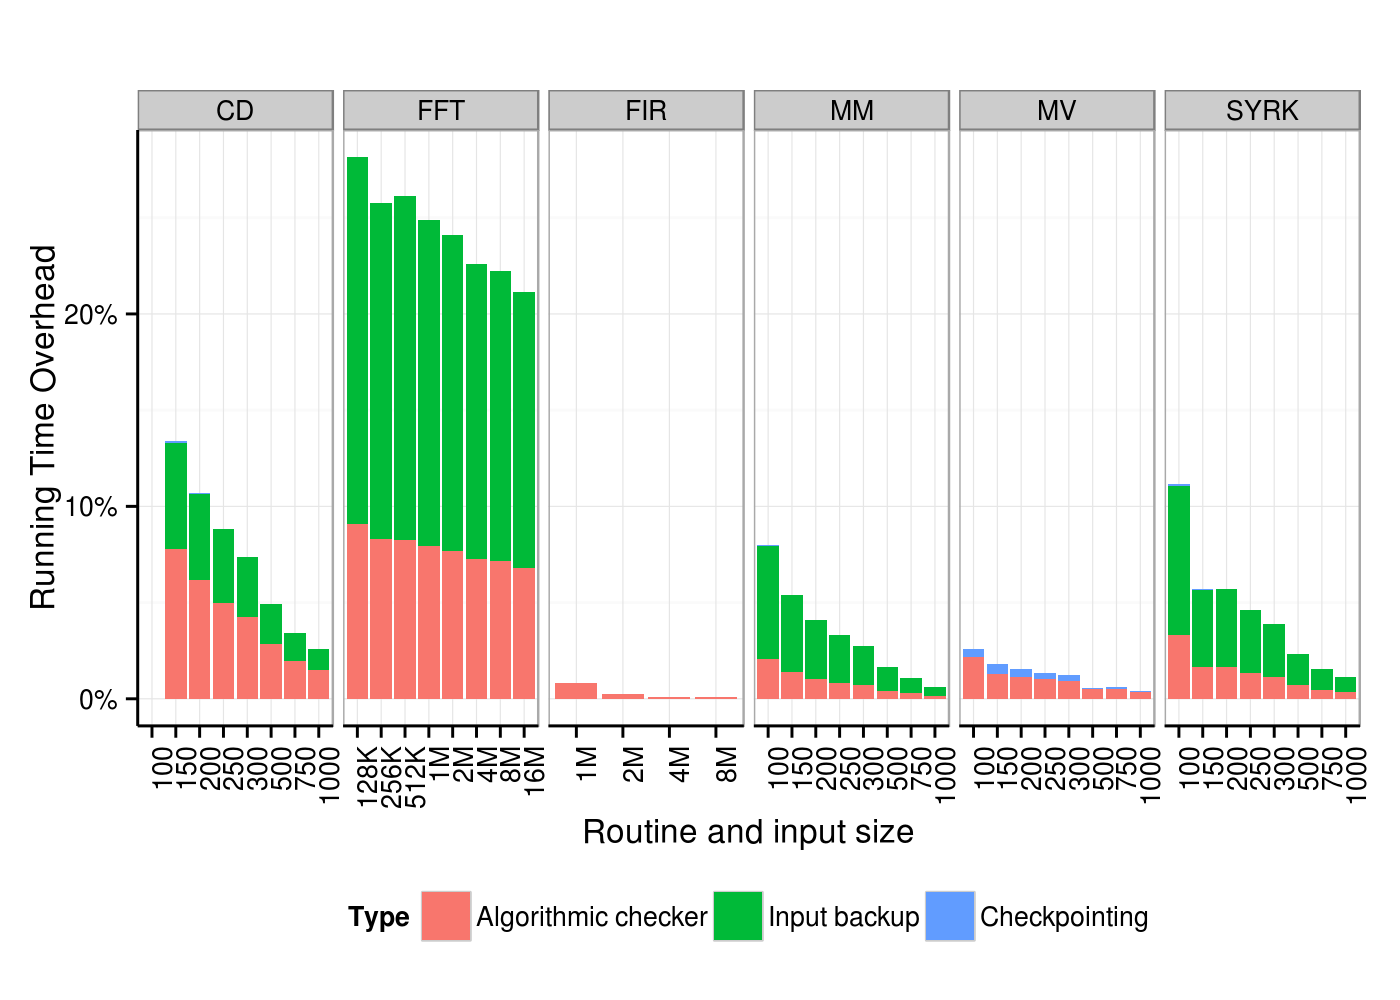
\includegraphics[width=1.00\columnwidth]{figs/4_1_1_Overall_Breakdown.png}
%\vspace{-5pt}
\caption{Overhead of resilience techniques. Results when no errors are injected are shown.}
\label{fig:routine_all_ovhd}
\end{figure}

Figure~\ref{fig:routine_all_ovhd} reports the relative increase in running time of MM, SYRK, MVM, CD, FFT and FIR as their input sizes are varied and no faults are injected.
MM, SYRK, MVM and CD were executed on square matrixes.
%The linear algebra routines were executed on $n \times n$ square matrices where $n$ varies from 100 to 1000.
%FFT ran on inputs vectors with 128K to 16M entries and FIR on window widths of 1M to 8M.
The experiments show that algorithmic error detection has a low overhead ($<10\%$) that shrinks with increasing input sizes.
The cost of checkpointing inputs is typically somewhat higher but also shrinks with increasing input size.
Checkpointing processor state (\texttt{sigsetjmp}) has a negligible cost.

\greg{Where is data for RK}
%RK ran on an integral with intervals $[0, t_1]$ where $t_1 \in \{10, 15, 20, 25, 30, 50, 75, 100\}$.
%Its ODE system is a second-order nonlinear Van der Pol oscillator equation.

\begin{figure}[ht!]
\centering
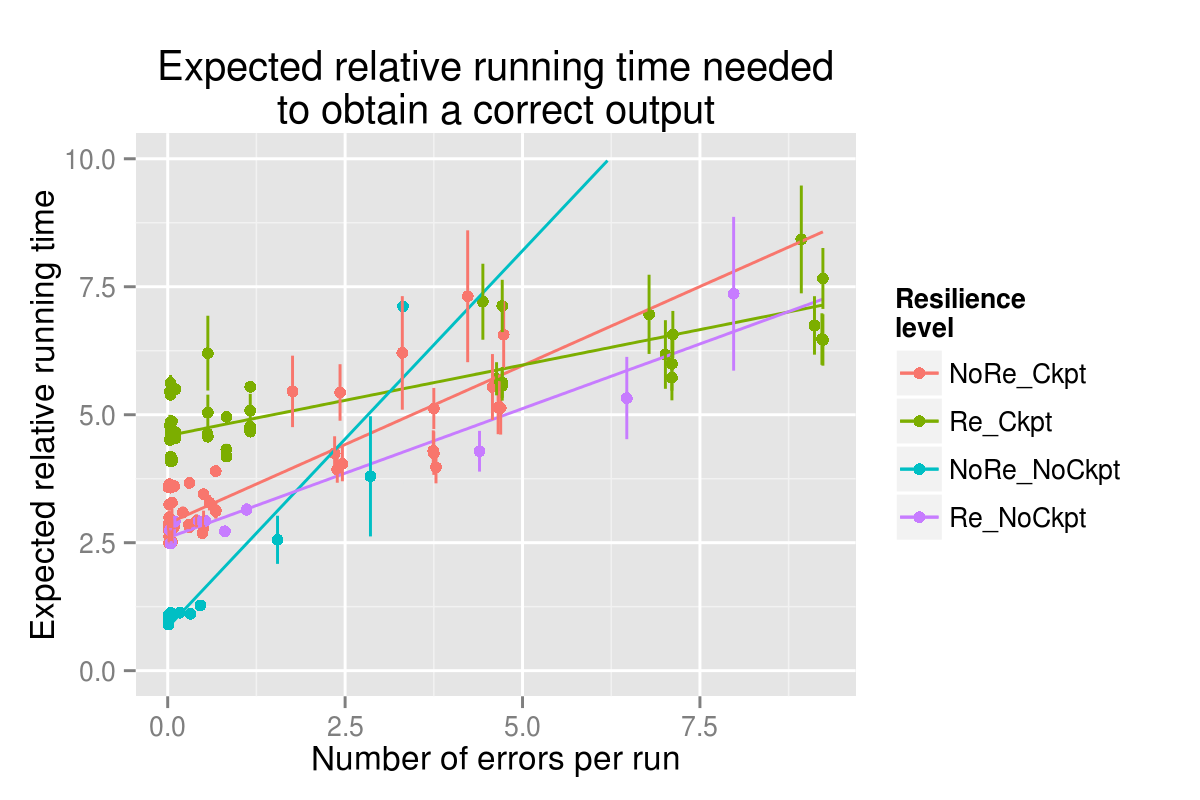
\includegraphics[width=1.00\columnwidth]{figs/4_1_2_Exp2_Expected_Running_Time_Needed.png}
\caption{Overhead of resilience techniques for RK when errors are injected}
\label{fig:rk_routine_exp_exec}
\end{figure}

When errors are injected there is an additional cost of rolling the computation back due to error detections.
Figure~\ref{fig:rk_routine_exp_exec} shows the effect on RK (similar for other routines (\greg{is this true})), when between 0 and 10 errors per run are injected and RK is protected using Checkpointing, Replication or both.
(\greg{What type of replication was used and what checkpointing period?})
The data shows that the best configuration varies with the number of errors.
\texttt{NoRe\_NoCkpt} (no resilience) is the most efficient option when only a few errors are injected but above 2.5 errors per run this configuration is aborted and restarted so often that resilience techniques are needed to achieve the best performance.
Replication without checkpointing is more effective than checkpointing without replication and for large error counts (>8 per run), both must be used.

\subsubsection{Result Accuracy}
\label{sec:res_tech:eval:accuracy}

Even though an application may complete its execution, errors injected into its numeric state may produce incorrect output.
In each experimental configuration we measured the distribution of errors in application output, measured as the Root Mean Square (RMS) Error: $\sqrt{\sigma_i (x_i-x'_i)^2}/n$, where $x_i$ is the value of output element $i$ in a fault-free run, $x'_i$ its value in a fault-injected run and $n$ is the total number of output elements (e.g. size of the output matrix).

Figure~\ref{fig:algo_err_dist} shows a sample of our results, focusing on the linear algebra routines (restarted upto 5 times after an error detection).
It presents the probability distribution of the routine's results having errors of various magnitudes.
Each tile corresponds to a different routine (vertical order) and different algorithmic error detection threshold used (horizontal order).
Table~\ref{fig:algo_err_heatmap} specifies the exact threshold values used.
Within each tile the vertical axis corresponds different error rates.
The axis numbers are normalized to the execution time of the configuration with no resilience techniques (\greg{errors injected or not?}) and specify the average number of errors injected during this time period at this rate.
The horizontal axis corresponds to the error magnitude ranging from 1e-14 to 1e-1.
For each error injection count and output error magnitude we report the probability of the output having error of \emph{larger than} this magnitude as a different shade of gray, with darker shades indicating higher probabilities.
Thus, darker plots indicate that error injections make larger output errors more likely and errors $\ge$ a smaller magnitude are always less likely than errors $\ge$ a larger one (shades grow lighter from left to right).

As error count increases the probability of larger output errors rises.
Further, tighter (smaller) error detection thresholds reduce this probability.
Error distributions vary widely, with MM being most resilient to errors (the probability of having large errors is low) and CD least.
These experiments guide the choice of how each routine's resilience technique is configured to meet user-specified accuracy bounds.

Figures~\ref{fig:algo_err_dist} show the fraction of entries in the outputs of each routine (y-axis) that have an error of a given magnitude (x-axis) as error magnitudes span from 1e-14 to 1e-4.
This figure is a focused view on few representative cases (each routine run on a single input size and error injection rate) across different resilience configurations: no error detection as well as three error detection thresholds.
As the error magnitude increases the fraction of output entries with errors of that magnitude drops.
Importantly, the fraction of erroneous entries is reduced at all magnitudes as a result of error detection and restart.
Further, this reduction is more significant as the detection threshold shrinks since smaller magnitude errors are detected.

Figure~\ref{fig:algo_err_heatmap} shows the same information but for all experimental configurations: (i) input sizes as above (ii) error injection rates of 1e-7 to 1e-10.
The graph is a grid, with results for different routines listed vertically and different resilience configurations (no detection and the different detection thresholds shown in the table at the bottom) listed horizontally.
The graph for each routine and resilience configuration presents the curves from Figure~\ref{fig:algo_err_dist} as a heatmap.
The y-axis shows different routine input sizes and error injection rates, sorted according to the average number of error injections per non-fault injected run, in decreasing order from top to bottom.
The x-axis shows the different error magnitudes and the shade of each point is the fraction of the routine's entries that have a given error magnitude, with darker shades indicating more such entries (each shade corresponds to a fraction that is some power of 10).
Thus, each row of Figure~\ref{fig:algo_err_heatmap} represents the same information as each curve in Figure~\ref{fig:algo_err_dist}, with the shades of the squares representing the same information as the height of the line's points.

%\begin{figure}[ht!]
%\centering
%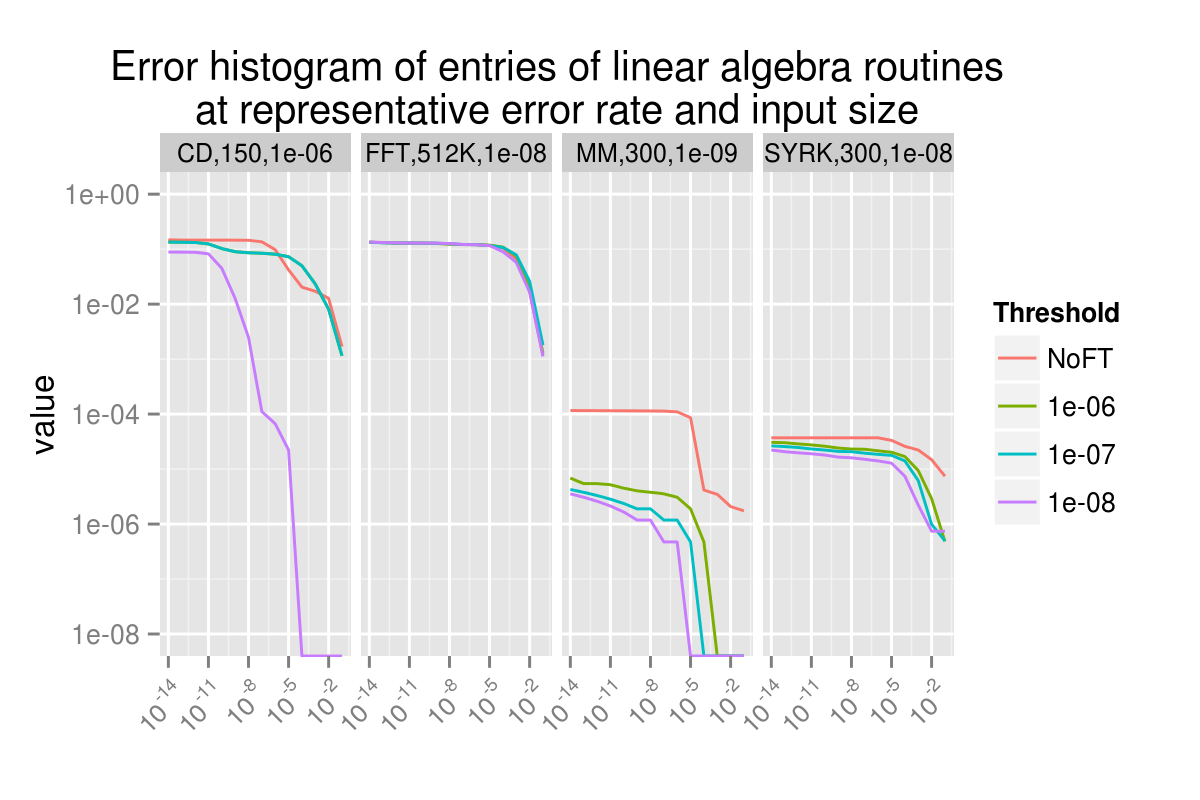
\includegraphics[width=1.00\columnwidth]{figs/4_1_1_Exp2_1_Example.png}
%\caption{Error magnitude histogram showing the effectiveness of the error detector}
%\label{fig:algo_err_dist}
%\end{figure}

\begin{figure}[ht!]
\centering
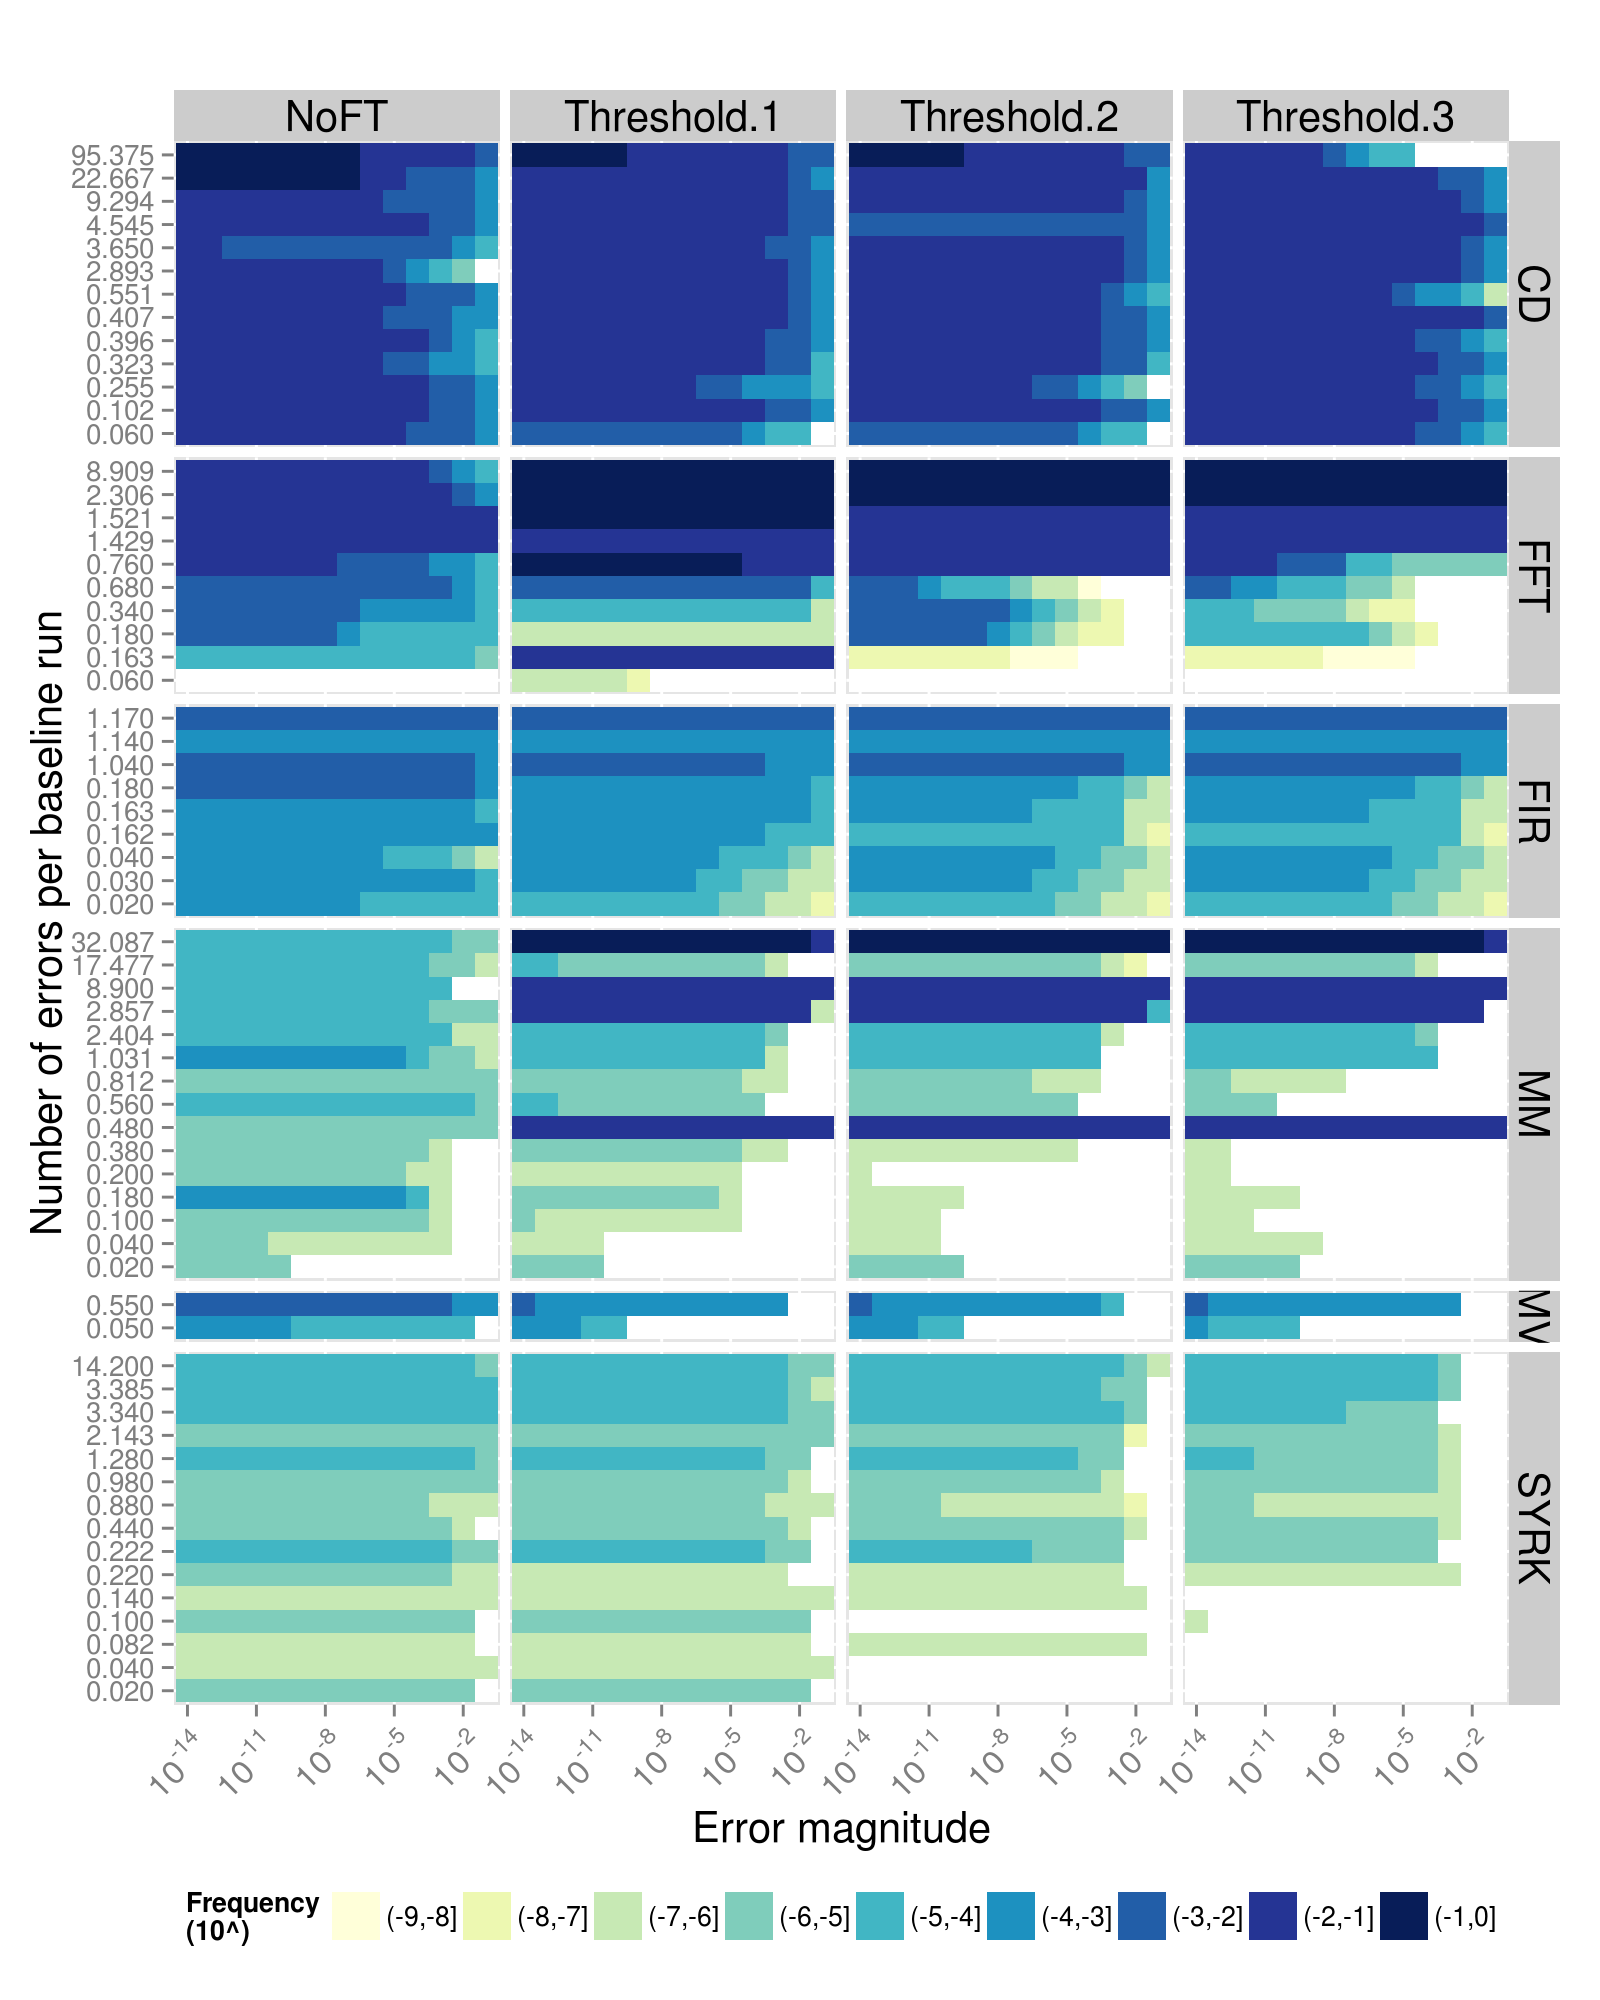
\includegraphics[width=1.00\columnwidth]{figs/4_1_1_Exp2_2_Heatmap_Error_ConfSpace.png}
\begin{tabular}{|p{0.5in}|p{0.7in}|p{0.7in}|p{0.7in}|}
\hline
Routine & Threshold 1 & Threshold 2 & Threshold 3 \\
\hline
\hline
CD & 1e-06 & 1e-07 & 1e-08 \\
\hline
FFT & 1e-06 & 1e-09 & 1e-14 \\
\hline
FIR & 1e-06 & 1e-09 & 1e-14 \\
\hline
MM & 1e-06 & 1e-07 & 1e-08 \\
\hline
MV & 1e-06 & 1e-07 & 1e-08 \\
\hline
SYRK & 1e-06 & 1e-07 & 1e-08 \\
\hline
\end{tabular}
\caption{Error magnitude histogram of the entire configuration space}
\label{fig:algo_err_heatmap}
\end{figure}

\section{Evaluation of Resilience Methodology in Applications}
\label{sec:eval}

To effectively and efficiently protect applications from soft errors we must consider each application's and routine's unique resilience needs as well as the user's accuracy requirements, the error rate of the hardware and the scale at which the application run (total execution time and number of compute cores).
We now build upon the analysis of individual routines summarized in Section~\ref{sec:res_tech:eval} to show how our methodology can be applied in the context of large-scale HPC applications.
The most accurate way to configure a large-scale application run on a given platform with a given input is to conduct a thorough fault injection campaign at this scale, injecting large numbers of errors into various code regions and processors.
Since this would require thousands of times more compute hours than a single large-scale application run, the only practical option is to extrapolate from small-scale application executions to large-scale ones.
This case study addresses this challenge by modeling large-scale instances of linear solver, signal processing and n-body simulation applications as combinations of small instances of these applications, that can indeed be comprehensively studied via a fault injection campaign.

This section reports the anticipated behavior of large-scale (1 million CPU-hours) runs of applications in these three domains.
We begin by describing our methodology to extrapolate the fault injection results for individual small-scale runs of ADDR, DRC and Hattrick to large-scale runs that connect many small-scale instances in various parallel and sequential dependence patterns.
We then apply analysis methodology described in Section~\ref{sec:res_tech:eval} to each of the three applications on various small-scale inputs to relate the various hardware error rate and the configurations of their resilience mechanisms to the resulting overhead and distribution of output errors.

The results of these experiments are used to select the most efficient configuration of the resilience mechanisms for each given hardware error rate and user accuracy requirement, focusing on the specific use-case of application runs that use 1 million CPU hours.
User accuracy requirements are expressed as a cap on the RMS error an application output may have and a bound on the probability with which this bound may be violated.
Since users rarely have a clear idea of how much RMS error is acceptable, we provide an alternative way to specify such bounds in terms of the amount of uncertainty about the application's inputs that would have generated a given amount of RMS difference between outputs.
By expressing the effects of soft faults using the same concepts as measurement error, this representation makes it easier to select an appropriate output accuracy and predict the effects of a given selection on other software that reads the application's output.


\subsection{Extrapolation Model}
\label{sec:eval:extrapolation}

Figure~\ref{fig:extrapolations} illustrates how individual runs of ADDR, DRC and Hattrick are combined to model large-scale instances of linear solver, signal processing and n-body simulation applications.
We observe that most large-scale applications can be described simple dependence graphs of identical tasks, such as the execution of a single time-step calculation in a single point in space.
The shape of the graph controls its total execution time and the way errors propagate.
Our model focuses on two major types of task graphs: parallel reduction and sequential chaining.

In the parallel reduction model all tasks run in parallel and their results are reduced into a common aggregate.
As such, the total execution time of the graph is the maximum execution time of all the tasks (approximated as the top 10 percentile as discussed below).
The RMS error of the aggregate is the combination of the RMS errors of the individual task outputs, which depends on the exact aggregation operation used.
Since averaging is a very common but not universal aggregation operation, in reductions we model the RMS error of the aggregate as the average of the RMS errors of individual tasks, which is an over-estimate of the RMS errors of their average.
In the sequential chaining model each task's output is used by the next task, forcing them to run in sequence.
The total execution time of task chains is thus the sum of the execution times of the individual tasks.
Tasks may either amplify or dampen errors in their inputs (output errors may be larger or smaller, respectively).
Given the complexity of dampening and amplification behavior that may occur in practice our model assumes that no dampening or amplification occurs and the error at the end of a task chain is equal to the maximum error of any task within the chain (also approximated as the top 10 percentile).

\greg{TODO: In addition to pure parallel and pure sequential dependence graphs we also considered sequences of parallel reductions, with the number of tasks in a given reduction equal to the number of reduction steps.}

\begin{figure}[ht!]
\centering
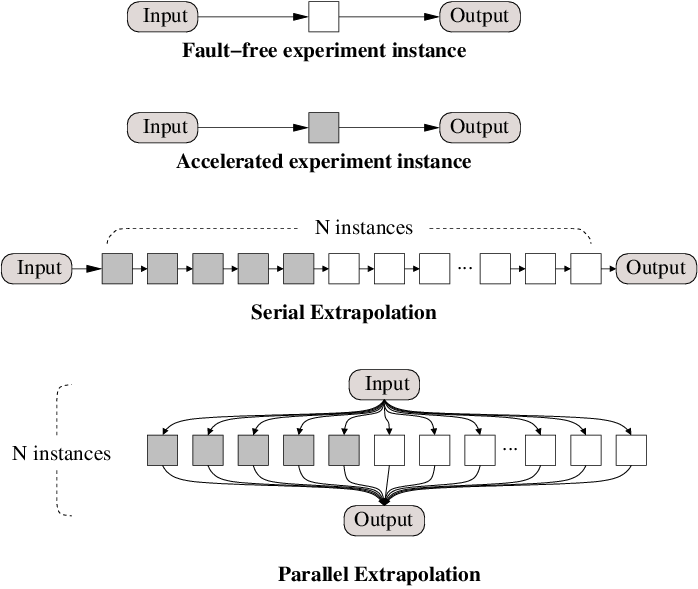
\includegraphics[width=1.00\columnwidth]{figs/extrapolates.png}
\caption{Extrapolation models}
\label{fig:extrapolations}
\end{figure}

We model large-scale linear solvers as dependence graphs of individual runs of ADDR, signal processing applications in terms of runs of DRC and n-body simulations in terms of runs of Hattrick.
Our experiments were performed on compute nodes with two 2.33 GHz dual-core Xeon E5345 processors with 4GB Ram and RHEL 4 Linux.
We run ADDR, DRC and Hattrick no fault injection on the inputs described in Section~\ref{sec:apps} and configuration options listed in Table~\ref{tbl:configs} to measure their fault-free execution time.
We also executed each configuration while injecting faults at rates to produce one or more injections per run.% (since different configurations have different execution times, the number of injections per run varies).
\greg{Since some runs
In each accelerated fault injection experiment, we ran each application configuration to completion, recording whether it completed and if so, the magnitude of the
	error.
	We calculate the execution time of each configuration, accounting for restarting the application in cases of unrecoverable failures via the formula $\frac{t_c}{1-p_f}$, where $t_c$ is the average completion time of such runs and $p_f$ is the probability of an unrecoverable failure.}
For each combination of application, input and configuration we performed 100 fault injections, for a total of 66,100 fault injection experiments for ADDR (4-process parallel runs), 43,200 for DRC (sequential runs), 102,000 for Hattrick (sequential runs).
For reference, assuming a typical FIT of 100-100,000 for individual processing cores (FIT = failure in one billion hours of operation and this range has been experimentally observed for commodity electronics~\cite{mem_errors:2010, dram_error:2009}), an HPC system with one million cores will experience .1-100 errors per hour, which is equivalent to 3e-11 - 3e-14 errors per processor cycle on a 1Ghz processor.
To make our analysis comprehensive we consider error rates between 1e-10 and 1e-16 (\greg{is this right?}).

We model the RMS error and expected execution time of a task graph that consists of executions of a given application, input and configuration combination (denoted a ``task''), on a system with a given per-processor error rate as follows.
Let $N$ be the total number of task runs needed to reach 1 million CPU hours and let $NF$ be the number of runs that are expected to have faults injected into them at the given error rate.
We sample $NF$ runs from the 100 fault injection runs conducted for the given configuration with replacement.
Replacement is used since faults are memory-less, they do not depend on prior faults.
As such, $NF$ may be larger than 100 without biasing the statistical results since the 100 runs are representative of the overall population.
We then add $N-NF$ copies of the non-fault injected variant of the given task to produce a complete sample of a large-scale application execution.
Finally, we compute the model application's metrics as:
\begin{eqnarray}
ExecTime_{Parallel} &= \text{Top 10 percentile of} ExecTime \text{of tasks in sample}\\
RMSE_{Parallel} &= \text{Average} ExecTime \text{of tasks in sample}\\
ExecTime_{Sequence} & = \text{Average} ExecTime \text{of tasks in sample}\\
RMSE_{Sequence} & = \text{Top 10 percentile of} ExecTime \text{of tasks in sample}
\end{eqnarray}
This procedure is repeated \greg{???} times to compute the expected value of the quantities.
We also use these samples to compute the 95\% confidence interval of the expected value (range where 95\% of the samples are located).

The reason why we use the top 10 percentile rather than the maximum is because the maximum metric is extremely sensitive to sampling.
Since there is no bound in the difference between the maximum of a given sample and the overall maximum, the only way to estimate it accurately is to sample the entire space of possibilities, which is prohibitively expensive.
In contrast, metrics such as average and percentiles are robust against such effects and can be accurately estimated from small samples.

\subsection{Intuitive Accuracy Metric}
\label{sec:eval:errorsensitivity}

Even in the absence of hardware faults scientific applications face many sources of error, including errors in input data, discretization error and modeling error.
All these sources of error are actively managed by application developers to ensure that the application's output remains useful.
Importantly, it means that hardware faults are only important if they cause errors larger than the ambient error that already exists in a given application, with a sufficiently high probability to make it a threat to decision-making.
While the probability of an inaccurate result makes intuitive sense to users, bounds on error are less intuitive and thus difficult to set.
As such, in this case study we relate output errors due to soft faults to measurement errors in application inputs, something that developers currently need to consider.
To this end we took the inputs to ADDR, DRC and Hattrick (all are matrixes or vectors of floating point numbers) and perturbed them by multiplying the values a random amount of noise sampled from a Gaussian distribution with mean 1 and a standard deviation that varies from 1e-9 to 1e0.
Figure~\ref{fig:inputvarianceoutputrmsd} shows the RMS difference (vertical axis) between the outputs of each application on every input, when noise with each standard deviation (horizontal axis) is and is not injected.
The data shows that DRC is largely insensitive to noise in its inputs, with RME differences of 1e-3 to 1e-2 typical across the noise spectrum.
This means that fault-induced RMS errors smaller than 1e-3 are completely irrelevant to this application and errors between 1e-3 and 1e-2 are typical for it.
In contrast, the output difference in ADDR and Hattrick are very sensitive to noise in the input, making it critical to set their target RMS error to be consistent with the uncertainty in the inputs.

\begin{figure}[ht!]
\centering
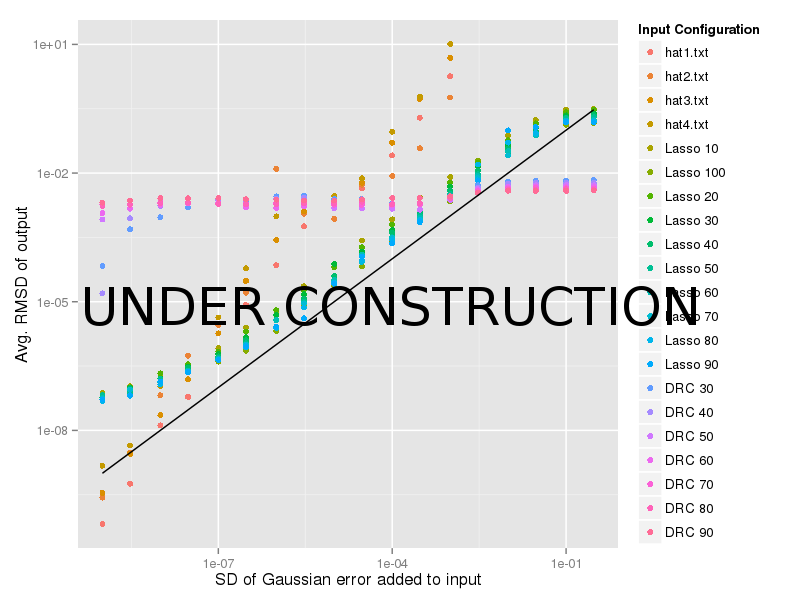
\includegraphics[width=1.00\columnwidth]{figs/InputVarianceOutputRMSD.png}
\caption{Extrapolation models}
\label{fig:inputvarianceoutputrmsd}
\end{figure}

%\subsection{Experiment setup}
%\label{sec:eval:confs}
%
%\sui{
%As we have seen in section \ref{sec:res_tech:eval}, varying the error checker thresholds in linear algebra routines and the checkpointing intervals and number of
%replicas in the RK4 integrator results in different levels of accuracy. As they are deployed in applications, choice of these parameters may influence how often
%the applications need to rollback in order to obtain correct results. An intuition is we should strike a balance between the tradeoff between correctness
%and performance. To explore the possible tradeoff in applications, we consider a range of parameters for our resilience techniques as described in section \ref{sec:res_tech:eval} when deploying the algorithmic checkers in these applications. The variable parameters and fixed parameters are listed as below.
%}
%
%\begin{figure}[ht!]
%\centering
%\begin{tabular}{|p{0.7in}|p{2.0in}|}
%\hline
%{\bf Application} & {\bf Resilience Techniques} \\
%\hline
%\hline
%Lasso & Checkers for MM, MV, CD, SYRK; input backup; protection for critical data structures \\
%\hline
%DRC & Checkers for FFT, FIR; input backup; protection for critical data structures \\
%\hline
%Hattrick & Checkpointing; protection for critical data structures; replication of pointers \\
%\hline
%\hline
%{\bf Application} & {\bf Variable Parameters} \\
%\hline
%\hline
%Lasso & Checker thresholds 1e-4 to 1e-7 \\
%\hline
%DRC   & Checker thresholds 1e-6 to 3e-8 \\
%\hline
%Hattrick & Checkpointing intervals 0, 1e3, 1e5; 0, 1, 2 replicas for each pointer \\
%\hline
%\end{tabular}
%\caption{Experiment Configurations}
%\label{fig:exp_confs}
%\end{figure}
%
%\sui{
%	In each accelerated fault injection experiment, we ran each application configuration to completion, recording whether it completed and if so, the magnitude of the
%	error.
%	We calculate the execution time of each configuration, accounting for restarting the application in cases of unrecoverable failures via the formula $\frac{t_c}{1-p_f}$, where $t_c$ is the average completion time of such runs and $p_f$ is the probability of an unrecoverable failure.
%}

% Configurations are described twice.
\subsection{Performance Impact}
\label{sec:eval:perf}
Figures~\ref{fig:Lasso_EstdCost}, \ref{fig:DRC_EstdCost} and \ref{fig:Hattrick_EstdCost} show the expected execution time \sui{of parallel (in dashed lines) and sequential (in solid lines) extrapolated instances}, relative to the execution time of the non-fault tolerant version of the extrapolation of the application when no errors are injected.

%Each figure shows a separate graph for each input size and along with the ID of the input shows the application's execution time on that input to quantify its vulnerability to errors on the input.
Data for the non-fault tolerant version is shown in red and the fault tolerant version with the optimal configuration for each input size is shown in blue.
The optimal configuration was selected to minimize overhead from across the following configuration spaces.

The graphs from left to right correspond to different application input sizes. Within each graph the x-axis corresponds to error injection rates (the real-system region of 3e-11 to 3e-14 highlighted in grey), while the y-axis shows the relative execution time. Both axes use logarithmic scales.

%For each configuration we plot a 95\% confidence interval.
%This is the range of relative execution times at the given error rate and application configuration in that will occur in 95\% of all trials.
%The confidence interval is computed by modeling the application's execution time as a Normal distribution.

Figure~\ref{fig:Lasso_EstdCost} shows that the non-fault tolerant ADDR slows down from 1.2x to 6x, depending on the input set size, as a result of the injected faults.
\sui{Although the fault tolerant version incurs overheads from the algorithmic checker and backing up input, the benefits from reducing the expected running time begins to outweigh the cost when the fault rate approaches 1e-11.} The optimal fault tolerance version the algorithm shows degradation that are around one half of the non-fault tolerant one \sui{when the fault rate exceeds 1e-10}, which implies that our technique improve ADDR's resilience by 50\%.
\sui{With the parallel extrapolation model, ADDR sees a higher running time overhead than with the serial extrapolation model. However it is much worth noting that as input size grows the overhead of the checkers become lower, as we have seen in section \ref{sec:res_tech:eval} with the individual linear algebra routines.}

Figure~\ref{fig:DRC_EstdCost}
%shows that since DRC performs many more integer operations and memory copies than ADDR, it is more vulnerable to errors that corrupt the values of pointers or cause loads and stores to target invalid memory locations.
\sui{shows that in DRC, the crossing point where the benefit fault-tolerant version outweights the cost of the algorithmic checker comes at a lower error rate than
that of Lasso. Just as we have seen in section \ref{sec:res_tech:eval}, the overhead from the algorithmic checkers become lower as the sampling rate increases.
Contrary to ADDR, DRC sees a larger overhead with the serial extrapolation model. This is because DRC is much more sensitive to input errors and is more likely
not to satisfy the user-specified error bound under the sequential extrapolation model than under the parallel extrapolation model.
}
%Such errors cause memory segmentation faults, which force DRC to restart its execution and thus incur a very high overhead.
%That is the reason why the performance slowdown of its non-fault tolerant version is much larger than for ADDR at high error rates.
%In contrast, the optimal fault tolerant version almost completely eliminates the performance impact of faults.
%However, at low error rates the cost of resilience is sufficiently high that at low error rates the non-fault tolerant version of DRC performs slightly better.

Figure~\ref{fig:Hattrick_EstdCost}
\sui{shows that the cost of pointer replication and checkpointing are almost negligible. Just as we see in DRC, this application sees a higher overhead with the serial extrapolation model than with the parallel extrapolation model, because the overhead induced by the fault tolerance mechanisms are
even smaller than those of DRC.
So, from these figures, we learn that
\begin{itemize}
\item{Under the sequential extrapolation model, the overhead of the application would mainly come from not being able to meet the error bound and having to roll back.}
\item{Under the parallel extrapolation model, the overhead of the application would mainly come from the overhead of the checkers themselves.}
\item{Whether the checker overhead or the roll-back overhead is more dominant is application-dependent.}
\end{itemize}
}

\begin{figure*}[ht!]
\centering
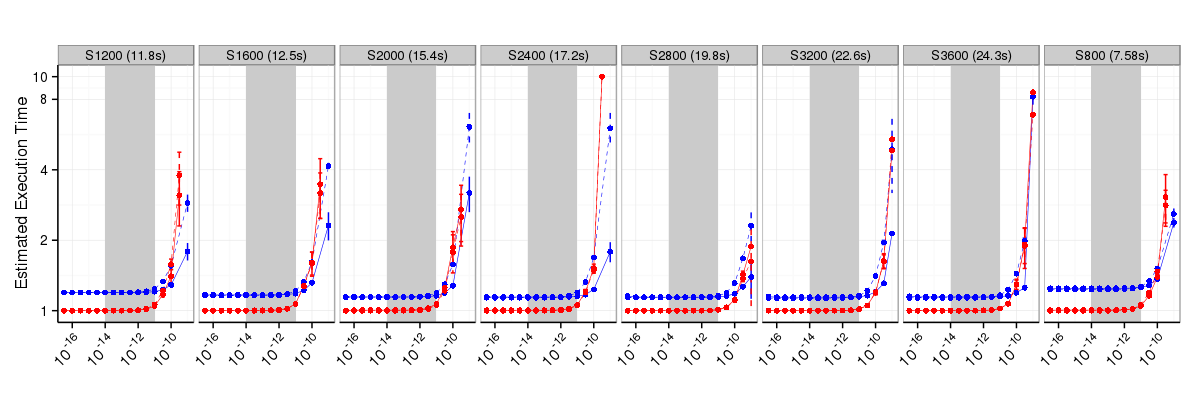
\includegraphics[width=7in]{figs/Lasso_Par_Seq_EstdCost_log.png}
\vspace{-10pt}
\caption{Execution time of ADDR relative to non-fault tolerant fault-free execution time. Results for the non-fault tolerant version (red) and the optimal fault tolerant version (blue) are shown.}
\vspace{-10pt}
\label{fig:Lasso_EstdCost}
\end{figure*}

\begin{figure*}[ht!]
\centering
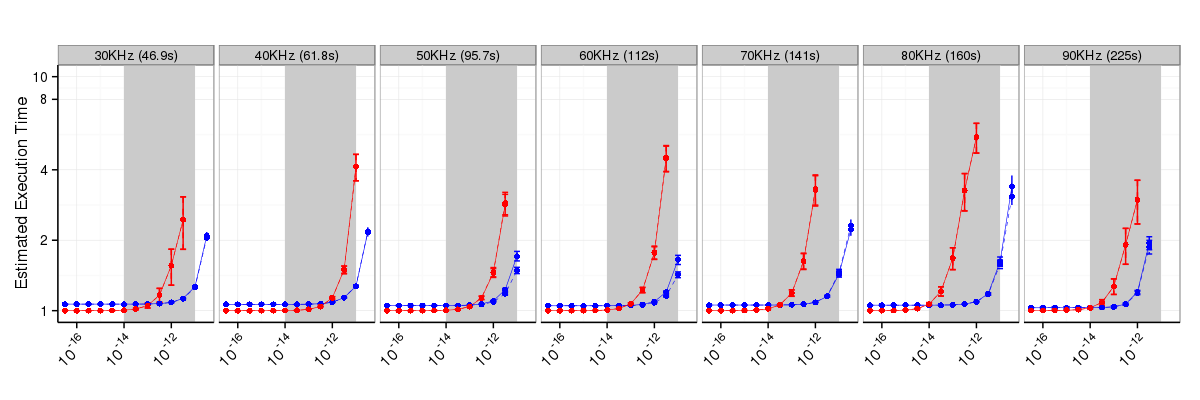
\includegraphics[width=7in]{figs/DRC_Par_Seq_EstdCost_log.png}
\vspace{-10pt}
\caption{Execution time of DRC relative to non-fault tolerant fault-free execution time. Results for the non-fault tolerant version (red) and the optimal fault tolerant version (blue) are shown.}
\vspace{-10pt}
\label{fig:DRC_EstdCost}
\end{figure*}

\begin{figure}[ht!]
\centering
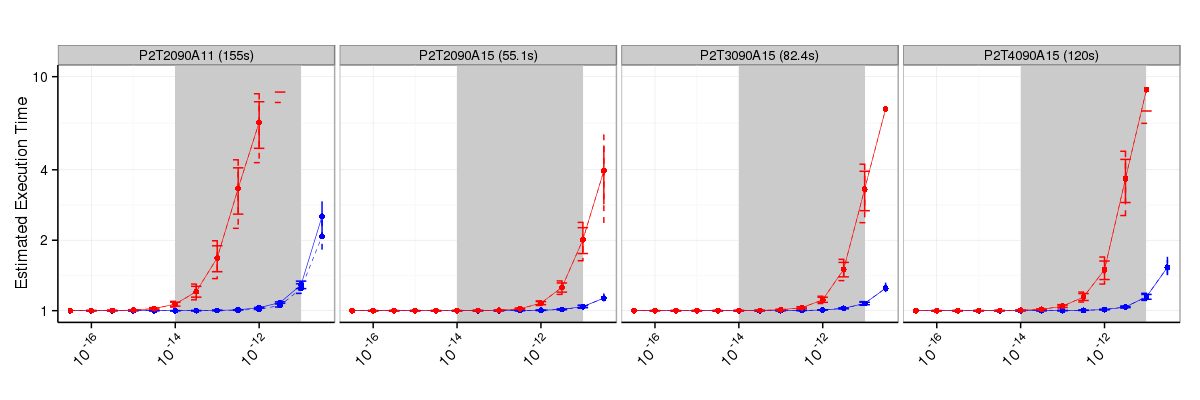
\includegraphics[width=3.4in]{figs/Hattrick_Par_Seq_EstdCost_log.png}
\vspace{-10pt}
\caption{Execution time of Hattrick relative to non-fault tolerant fault-free execution time. Results for the non-fault tolerant version (red) and the optimal fault tolerant version (blue) are shown.}
\vspace{-10pt}
\label{fig:Hattrick_EstdCost}
\end{figure}

%\sui{When a user wants to run an application under a faulty environment and obtain correct results, s/he would have to expect to run a part of this application multiple times in case the application aborts due to memory access errors or return useless incorrect results. The user might want to have the application return to a certain checkpoint, or restart the entire application should any unrecoverable occurs. The cost of rollback, and the chance of each type of errors occurs at a different rate. The Markov model comes into play here with its capability to capture all these parameters of experiments we have already run and predict the running time of the applications at configurations not experimented with.}


%Experiment 1: Measure the slowdown of each application at the optimal configuration
%Experiment 2: Measure the rate of aborts due to algorithmic errors, segfaults and redundant copy mismatches (separate the causes)

\subsection{Result Accuracy}
\label{sec:eval:acc}

%Experiment: Measure the accuracy of the results produced in completed runs, including error bars on the variability of the errors

This section evaluates the distribution of errors in the resulting outputs.
First of all, if the probability that a given run completes without an unrecoverable error is greater than 0 then the application will eventually complete with some output after some number of restarts. \sui{The restarts translate into the roll-back head reflected in section \ref{sec:eval:perf}.}

The accuracy is quantified in the following way:
The output of ADDR is the vector that holds the solution to the linear system.
For Hattrick it is the vector that holds the state of the n-body system at the final application time-step, with 6 numbers per body
Finally, DRC's output is a Pulse Code Modulation-formatted file, which is a sequence of numbers.
Since the outputs of each routine can be represented as a vector we calculate the error in the outputs by comparing the vector $v_e$ returned by each application when errors are injected to the correct vector $v_c$ computed during a fault-free run and computing the L2 norm of the difference: $\sqrt{\frac{\sum_{i} (v_c-v_e)^2}{\left| v_c \right|}}$.

Figures~\ref{fig:Lasso_ImperfectRate}, \ref{fig:DRC_ImperfectRate} and \ref{fig:Hattrick_ImperfectRate} show the errors in ADDR, DRC and Hattrick outputs from a user-centric perspective.
They plot the fraction of application runs for which a numerical error equal or smaller than $10^{-8}$ is achieved.
From left to right each figure shows graphs for different input sizes and from top to bottom it shows results for different error magnitude bounds.
The x-axis in each graph shows the fault injection rate while the y-axis shows the fraction of runs where the error target was satisfied.
Both axes are expressed in logarithmic scale.
Each graph shows data for the non-fault tolerant version of the application (all points connected by the line) as well as all the fault tolerant versions (optimal configurations connected by a line).
%The 95\% confidence interval is plotted and denotes the range of probabilities that the error bound will be achieved at the given error rate and application configuration in 95\% of all trials.
%It is computed by modeling the number of times application results will meet the error bound using a Binomial distribution.
%Given a binary random variable that is equal to 1 (i.e. error bound achieved) with probability $p$ and 0 (i.e. bound missed) with probability $1-p$ the Binomial distribution is the number of trials where it is 1.

The data shows that the probability that the non-fault tolerant version of each one the three application violates the user-provided error bound is above 10\% for Hattrick and DRC in the region of realistic error rates (3e-11 to 3e-14) and above 1\% for ADDR across all inputs.
When resilience is applied to these applications the probability of violating the error bound drops to below 1\% for ADDR and Hattrick and below 10\% for DRC in the same region.
\sui{And, not surprisingly, an instance under the parallel extrapolation model is more likely to meet the error bound than one under the sequential extrapolation model.}
This shows that the use of all the resilience techniques is critical for ensuring that application outputs are valid with a high probability even on very large HPC systems.


\begin{figure*}[ht!]
\centering
%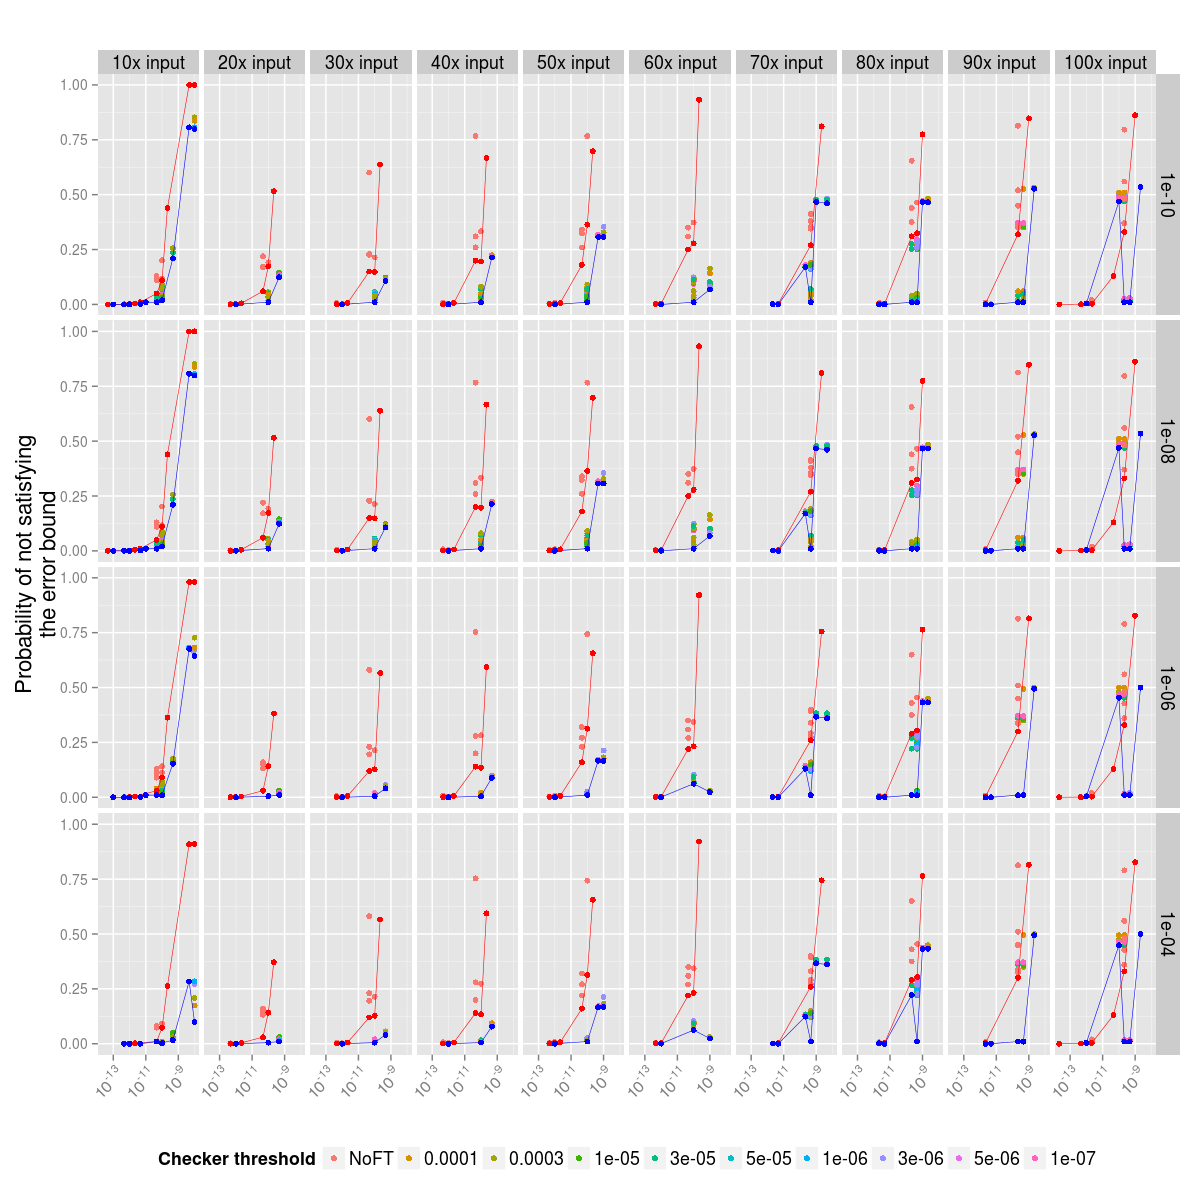
\includegraphics[height=5in]{figs/Lasso_ImperfectRate.png}
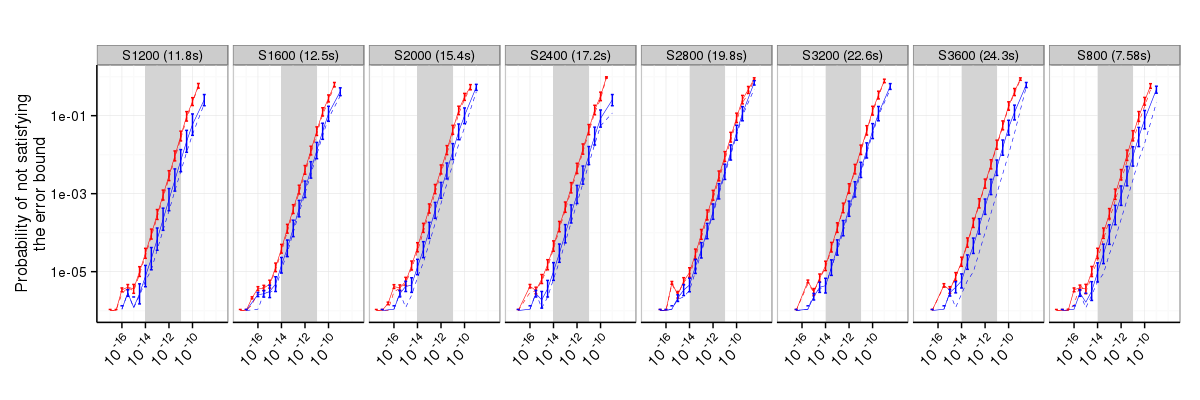
\includegraphics[width=7in]{figs/Lasso_Par_Seq_ImperfectRate_log.png}
\vspace{-10pt}
\caption{Probability of not satisfying the user-provided error bound for ADDR. Results for the non-fault tolerant version (red) and the optimal fault tolerant version (blue) are shown.}
\vspace{-10pt}
\label{fig:Lasso_ImperfectRate}
\end{figure*}

\begin{figure*}[ht!]
\centering
%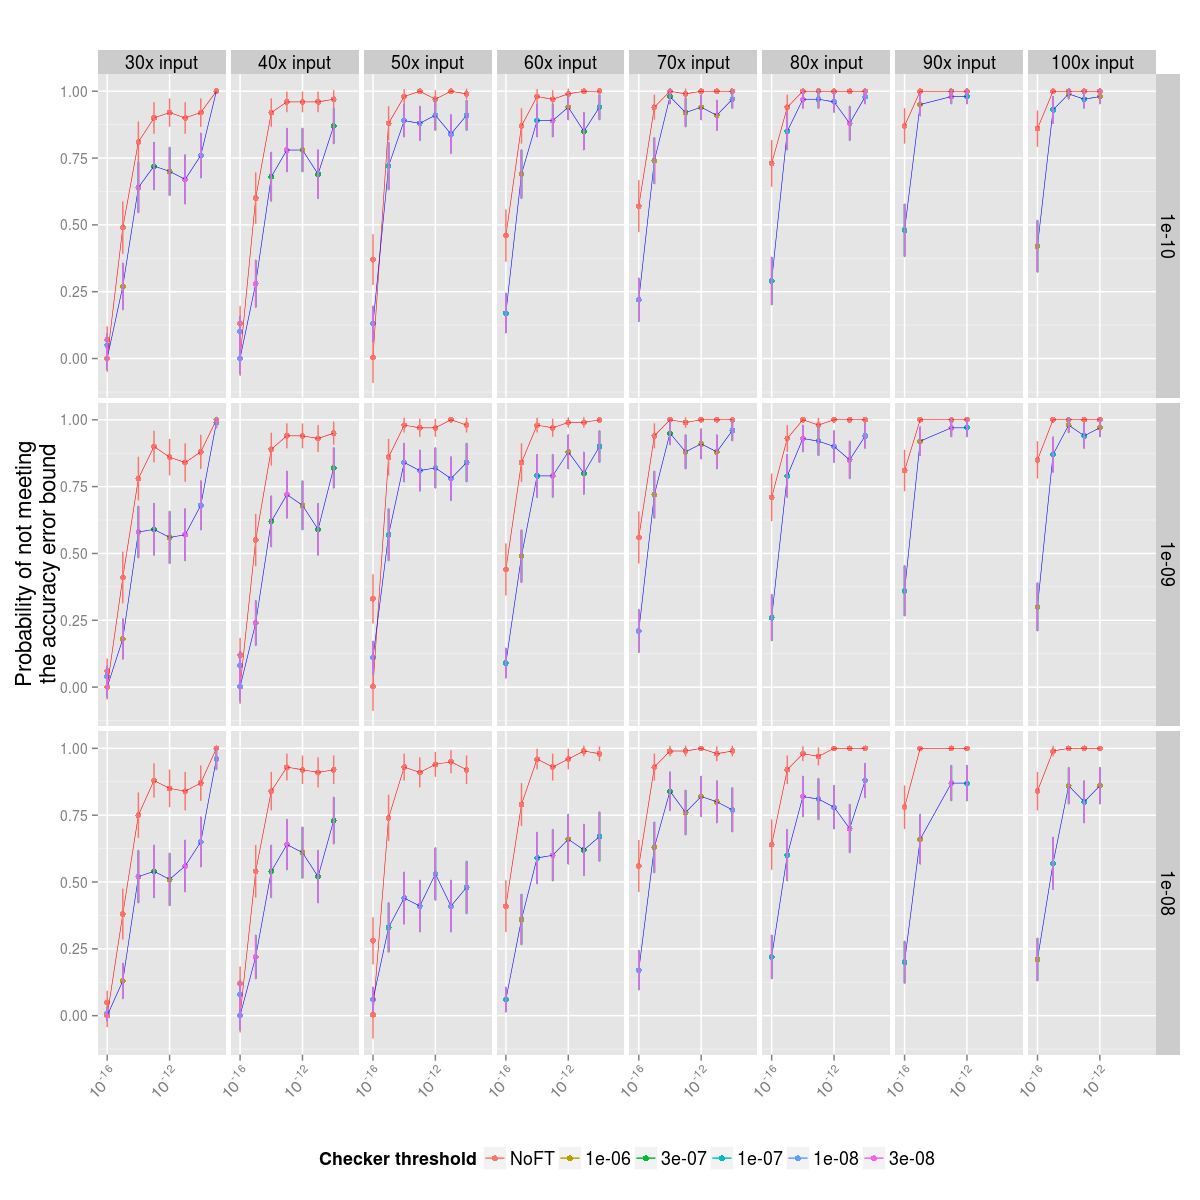
\includegraphics[height=3in]{figs/DRC_ImperfectRate.png}
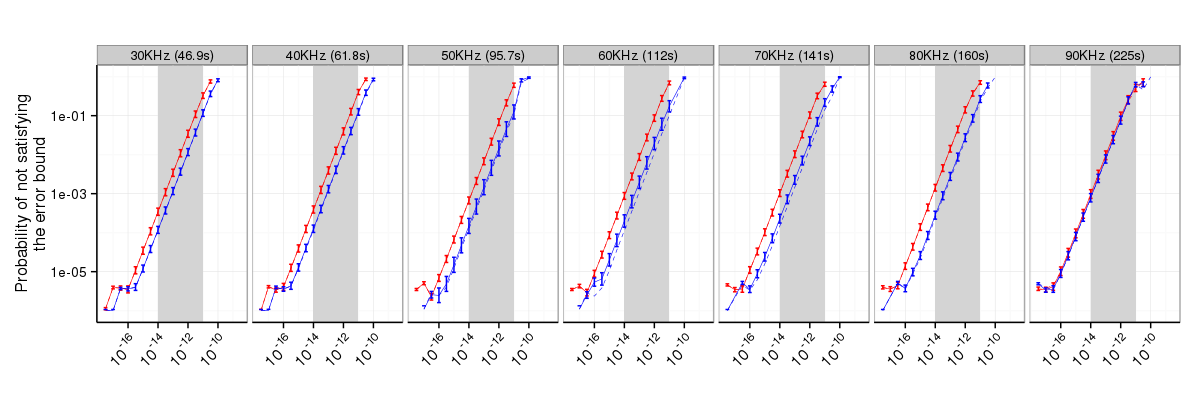
\includegraphics[width=7in]{figs/DRC_Par_Seq_ImperfectRate_log.png}
\vspace{-10pt}
\caption{Probability of not satisfying the user-provided error bound for DRC. Results for the non-fault tolerant version (red) and the optimal fault tolerant version (blue) are shown.}
\vspace{-10pt}
\label{fig:DRC_ImperfectRate}
\end{figure*}

\begin{figure}[ht!]
\centering
%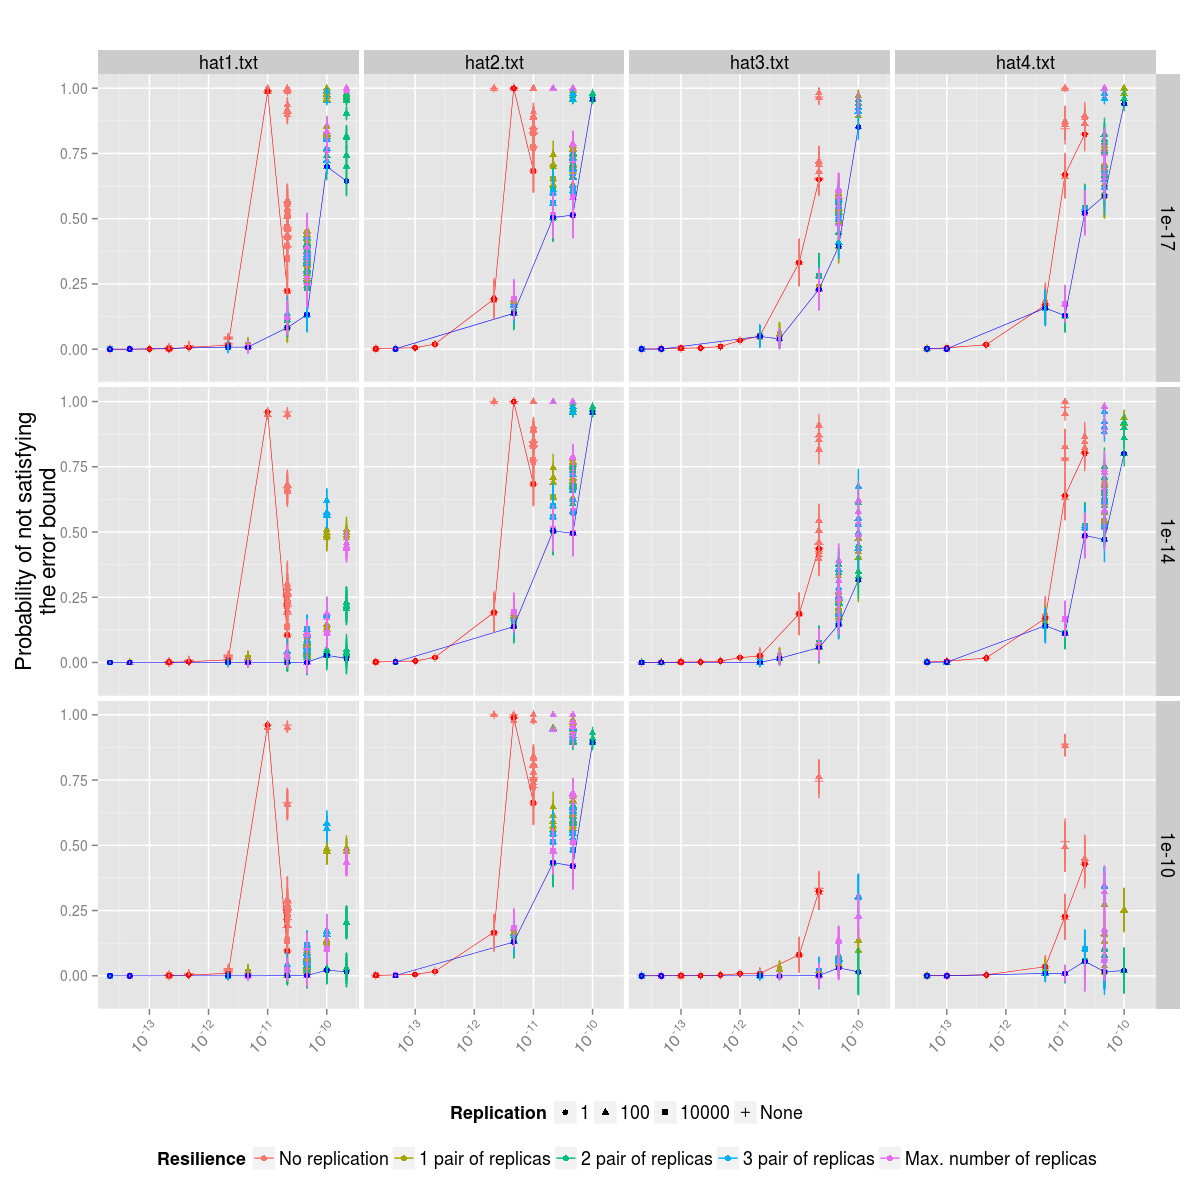
\includegraphics[height=3in]{figs/Hattrick_ImperfectRate.png}
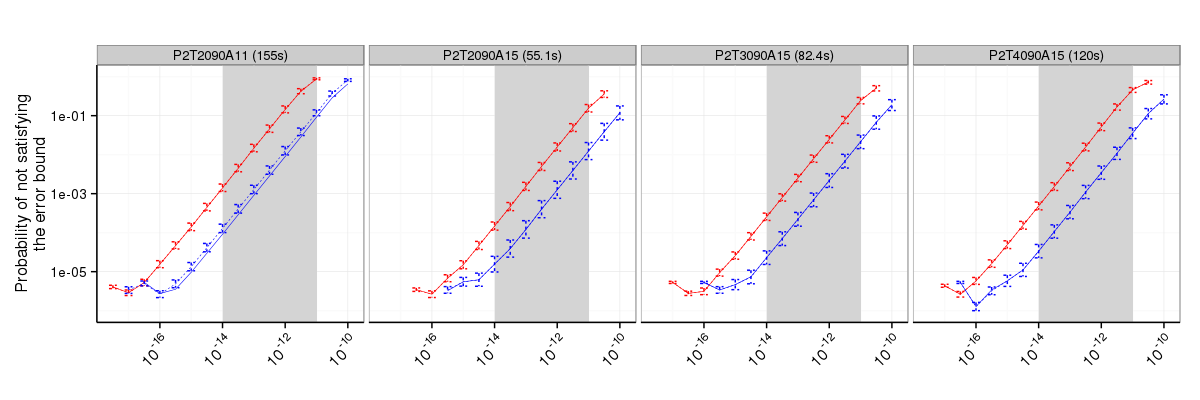
\includegraphics[width=3.4in]{figs/Hattrick_Par_Seq_ImperfectRate_log.png}
\vspace{-10pt}
\caption{Probability of not satisfying the user-provided error bound for Hattrick. Results for the non-fault tolerant version (red) and the optimal fault tolerant version (blue) are shown.}
\vspace{-10pt}
\label{fig:Hattrick_ImperfectRate}
\end{figure}

\subsection{Choice of Optimal Fault Tolerance Techniques}
\label{sec:eval:optchoice}

\sui{Figures XXX show the choice of optimal fault tolerance techniques in the parallel and sequential extrapolated runs of all three applications.}

\sui{(All Suggested Fault Tolerance Configuration figures)
There are cells in the figures that are not shaded. These cells mean there is not any possible fault tolerance configuration available to satisfy the user-specified probability of not satisfying the error bound because the specified probability is too low and error rate is to high.}

\sui{(All Probability of not satisfying user's error bound figures)
Serial extrapolated runs have a slightly higher than parallel extrapolated ones.}

\sui{(Comparing Lasso's Parallel and Serial Estimated Optimal Cost)
When error rates are low, the overhead of both serial and parallel fault-tolerant runs are dominated by the algorithm checker. By the nature of the error checkers, their overheads decrease as input size goes up.
As fault rate increases, the parallel run sees a more rapid gain in overhead than a serial run. This is because the overhead of rolling back the faulty runs becomes more pronounced in parallel runs than serial runs.}

\sui{(Comparing Lasso's Parallel and Serial Suggested Fault Tolerance Configurations)
From the cells that are shaded, as can be expected from the extrapolation model, a serial run requires a tighter error bound. }

\sui{(Comparing DRC's Parallel and Serial Estimated Optimal Cost)
Due to a much smaller proportion of the cost of rolling back in the samples of DRC, the difference between serial and parallel runs of DRC is much smaller than that of the serial and parallel runs of Lasso.}

\sui{(Comparing DRC's Parallel and Serial Suggested Fault Tolerance Configurations)
From the cells that are shaded, a serial run requires a tighter error bound.}

\sui{(Comparing Hattrick's Parallel and Sequential Estimated Optimal Cost)
Since the cost of Hattrick's checkpointing code is almost negligible, the difference between the performance overheads of the parallel and serial extrapolation models is also almost negligible.}

\sui{(Comparing Hattrick's Parallel and Serial Suggested Fault Tolerance Configurations)
From the cells that are shaded, a serial run requires a tighter error bound.}

\begin{figure*}[ht!]
\centering
%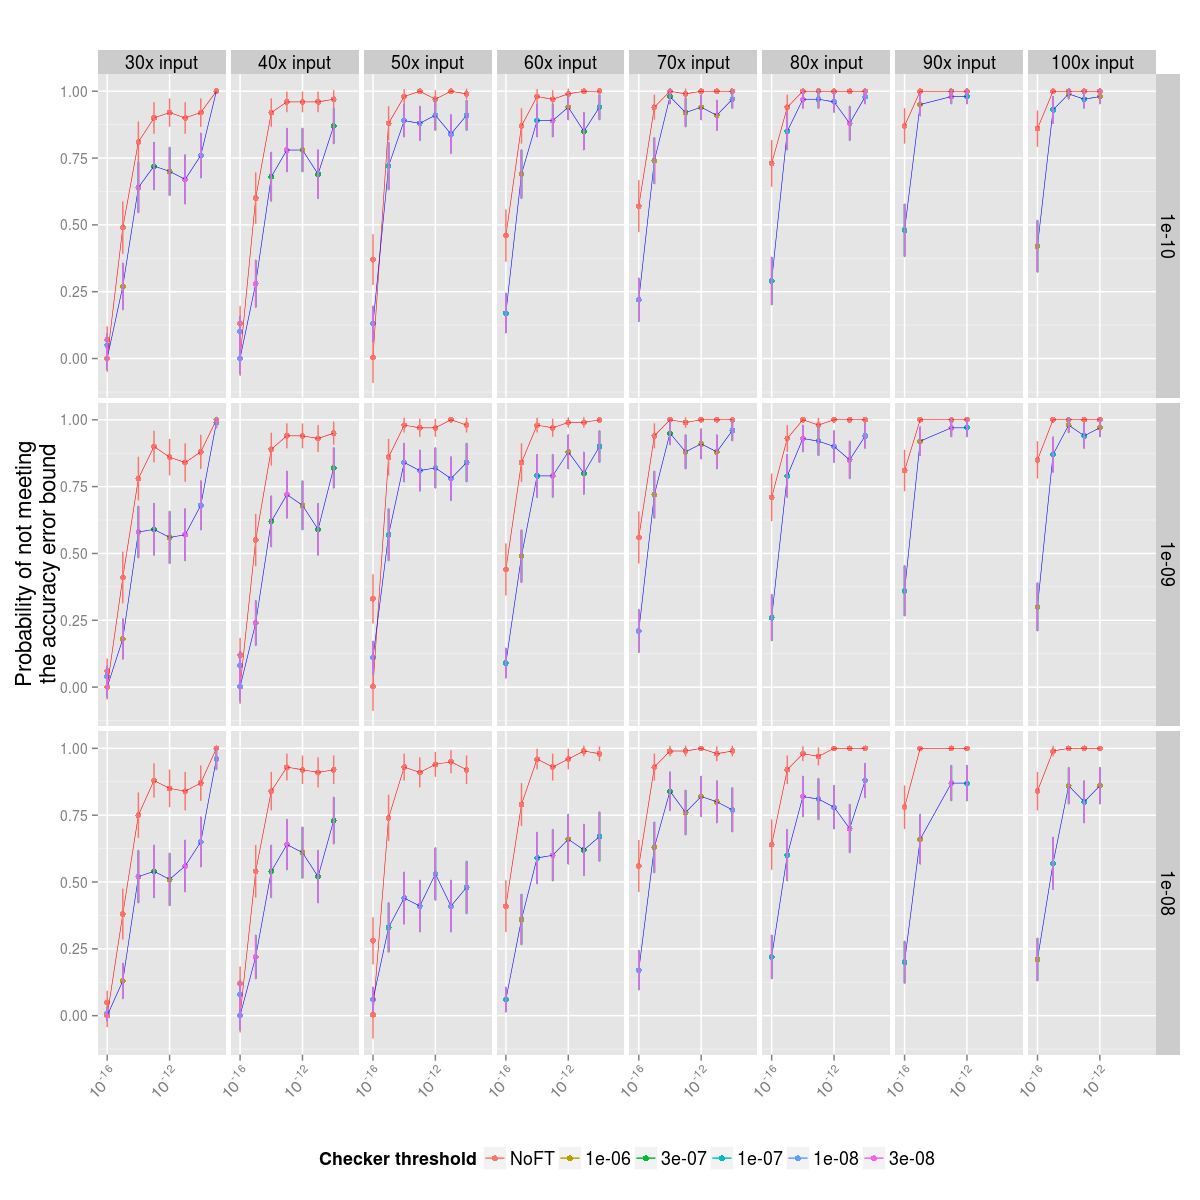
\includegraphics[height=3in]{figs/DRC_ImperfectRate.png}
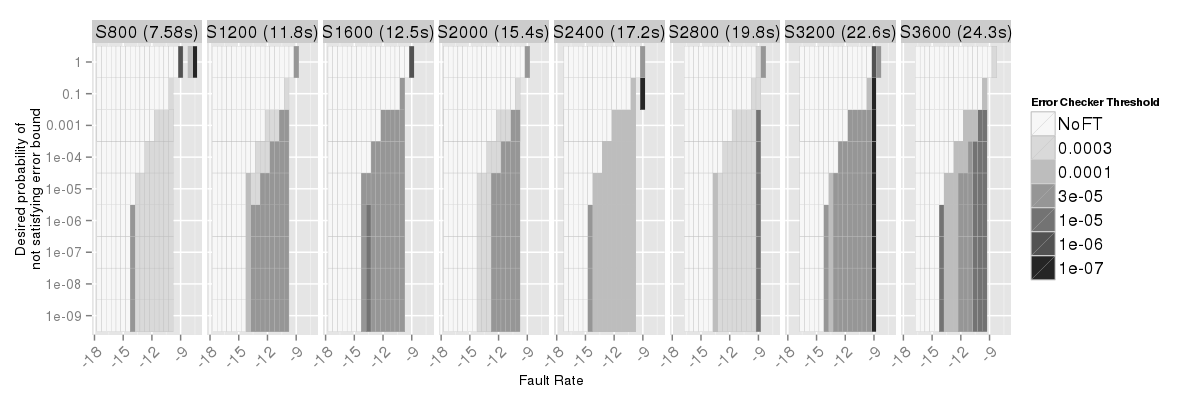
\includegraphics[width=7in]{figs/Lasso_Parallel_SuggestedConf.png}
\vspace{-10pt}
\caption{Suggested Resilience Technique for ADDR Under the Parallel Extrapolation Model Under Different Fault Rates}
\vspace{-10pt}
\label{fig:Lasso_Parallel_SuggestedConf}
\end{figure*}

\begin{figure*}[ht!]
\centering
%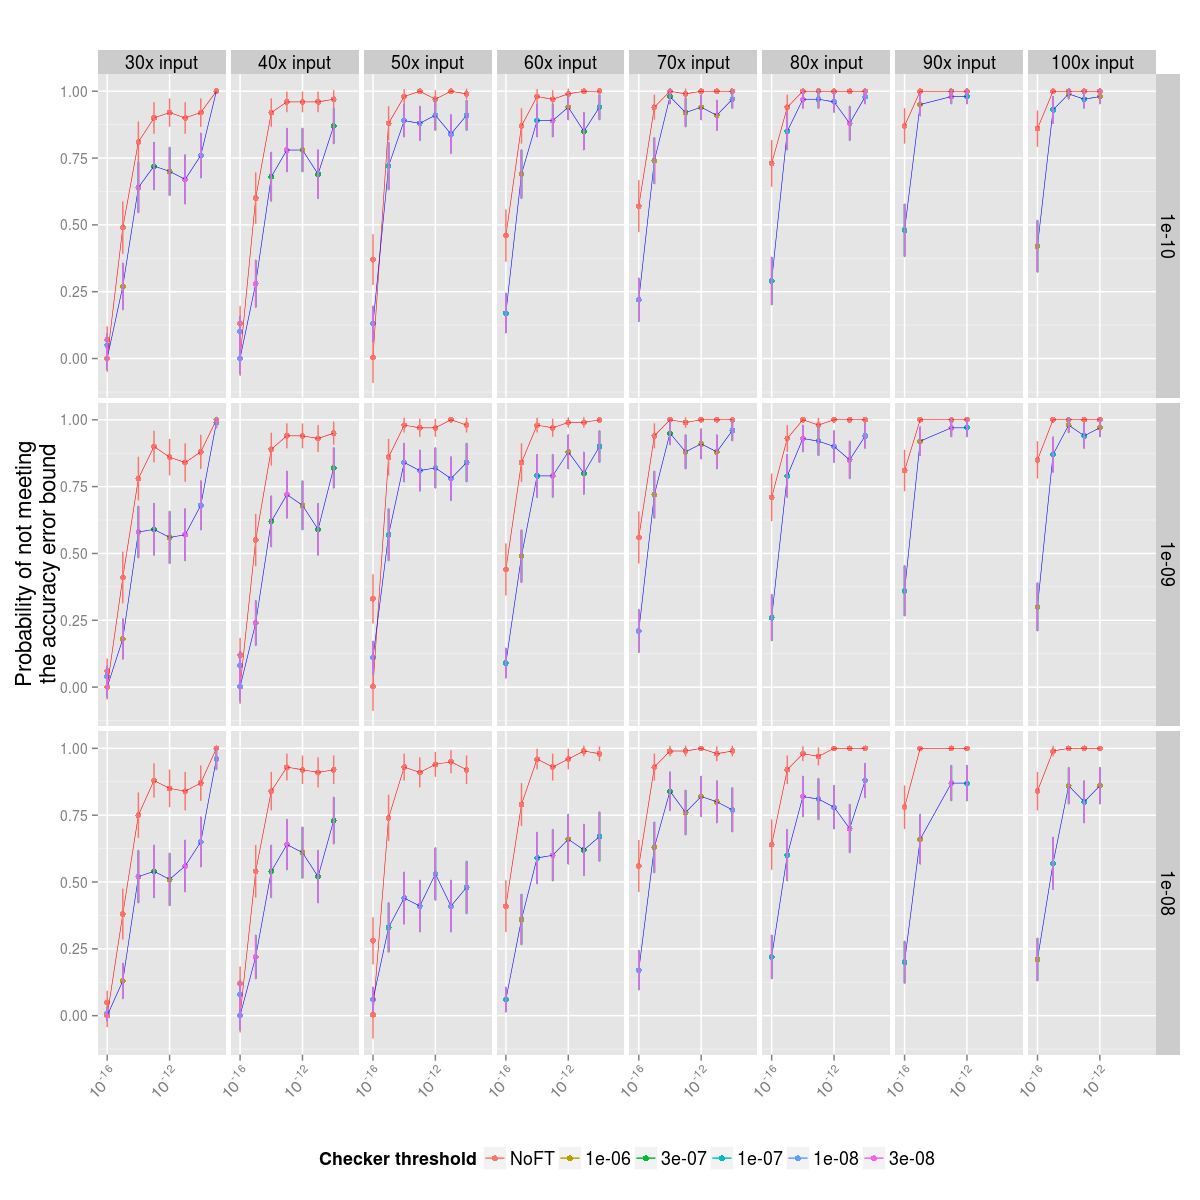
\includegraphics[height=3in]{figs/DRC_ImperfectRate.png}
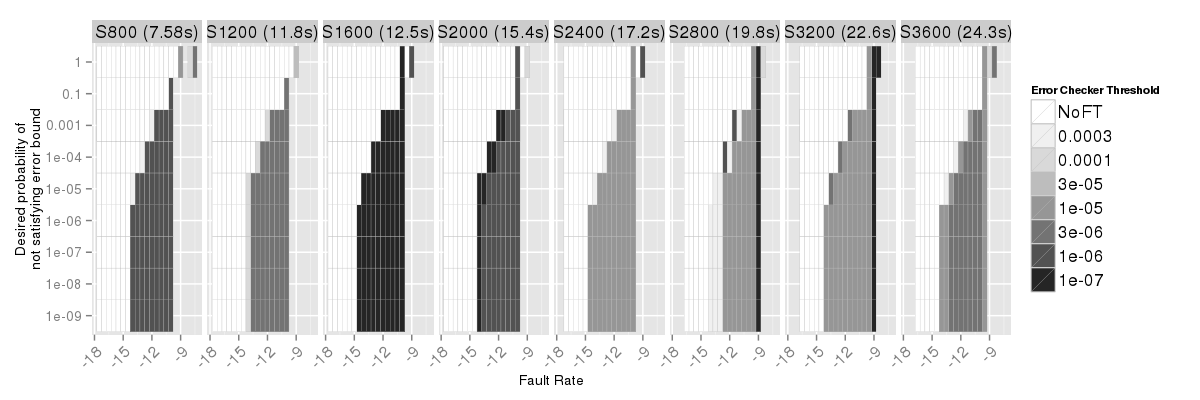
\includegraphics[width=7in]{figs/Lasso_Serial_SuggestedConf.png}
\vspace{-10pt}
\caption{Suggested Resilience Technique for ADDR Under the Serial Extrapolation Model Under Different Fault Rates}
\vspace{-10pt}
\label{fig:Lasso_Serial_SuggestedConf}
\end{figure*}

\begin{figure*}[ht!]
\centering
%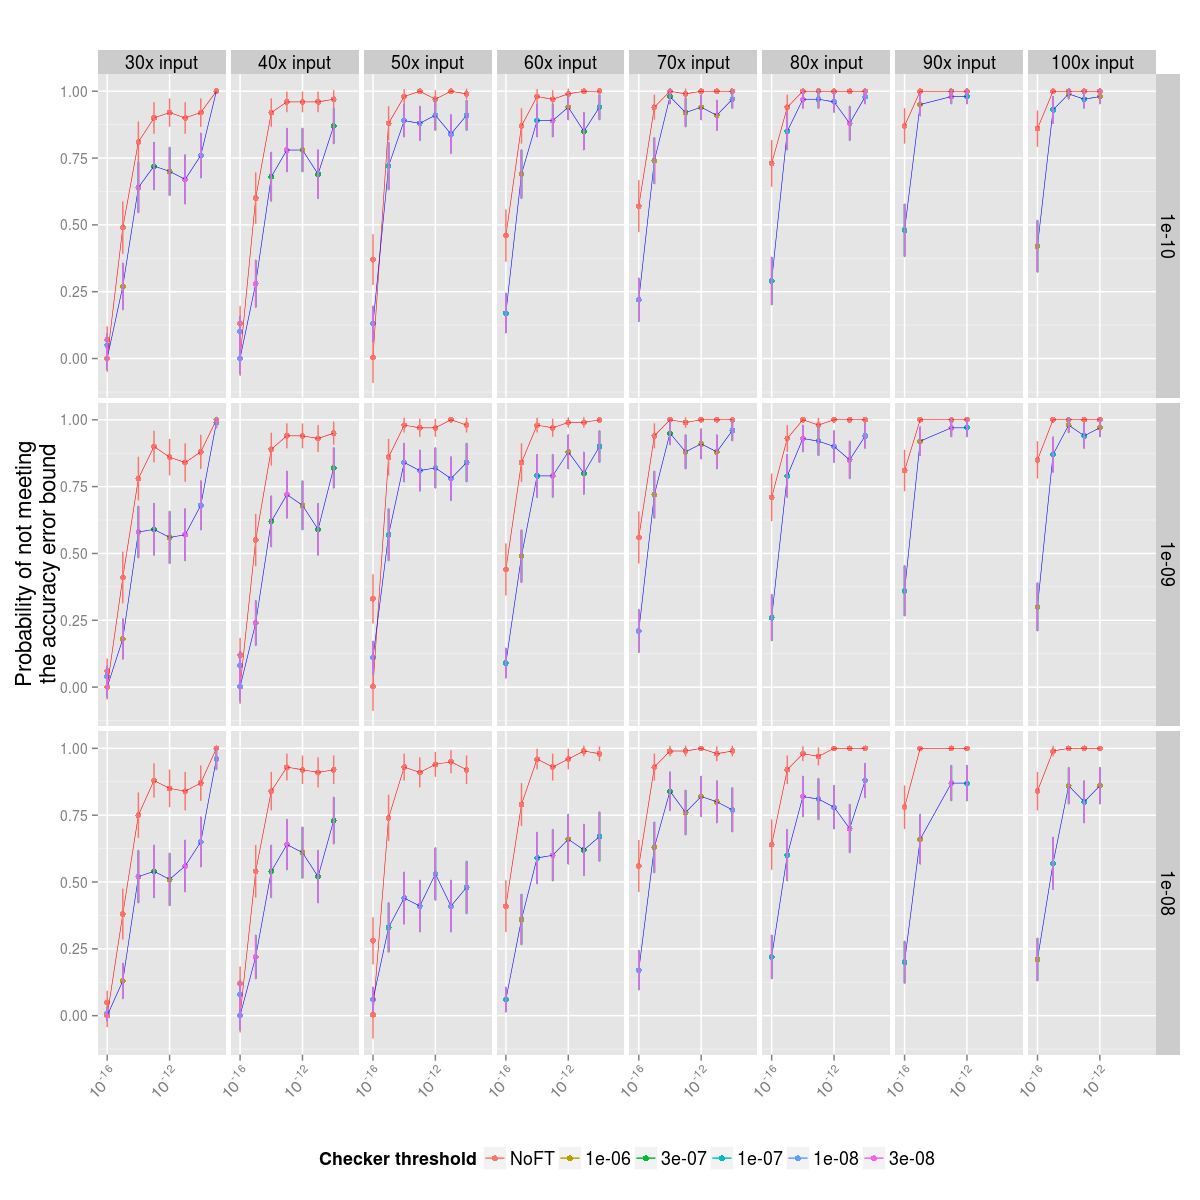
\includegraphics[height=3in]{figs/DRC_ImperfectRate.png}
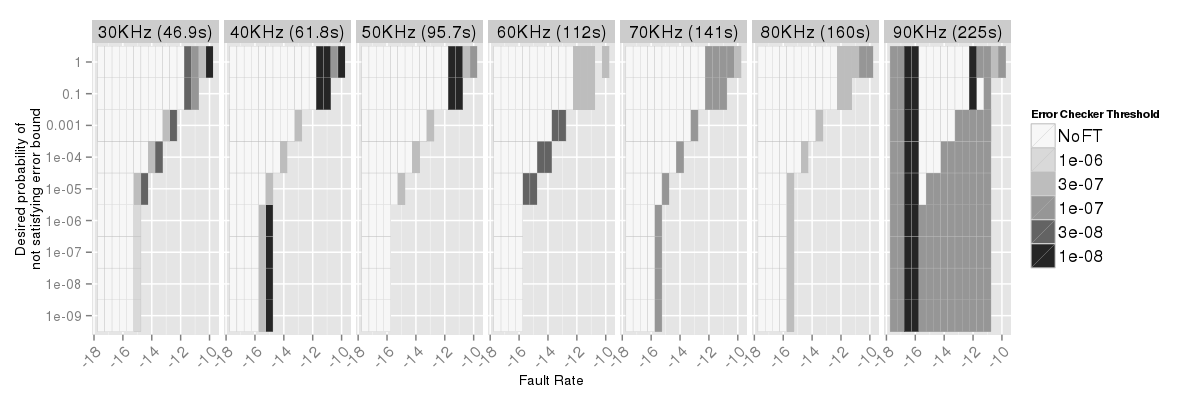
\includegraphics[width=7in]{figs/DRC_Parallel_SuggestedConf.png}
\vspace{-10pt}
\caption{Suggested Resilience Technique for DRC Under the Parallel Extrapolation Model Under Different Fault Rates}
\vspace{-10pt}
\label{fig:DRC_Parallel_SuggestedConf}
\end{figure*}

\begin{figure*}[ht!]
\centering
%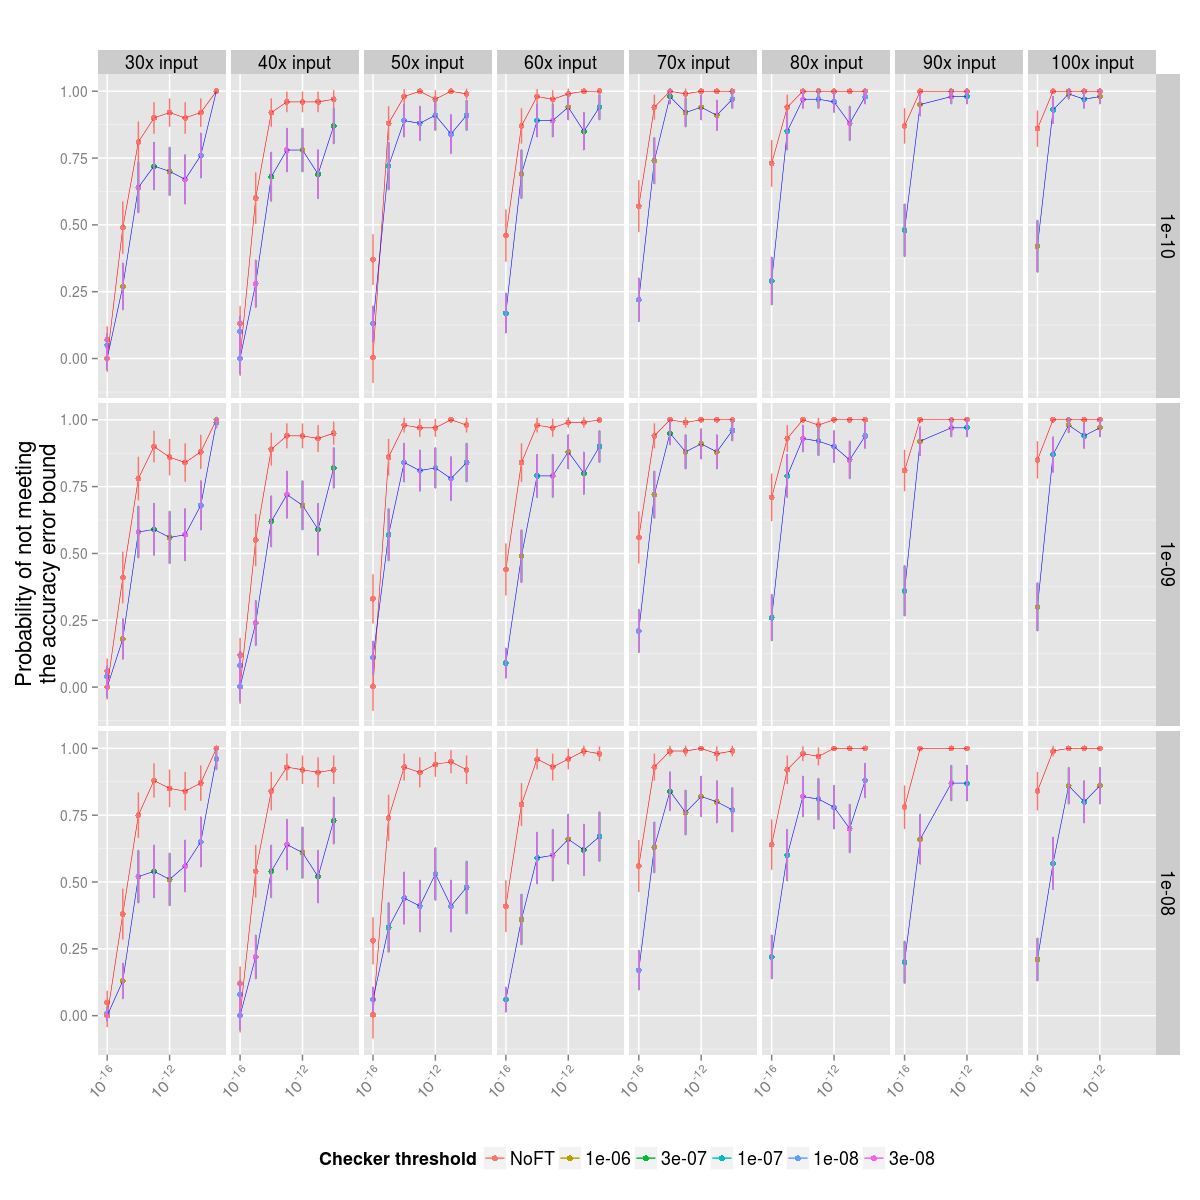
\includegraphics[height=3in]{figs/DRC_ImperfectRate.png}
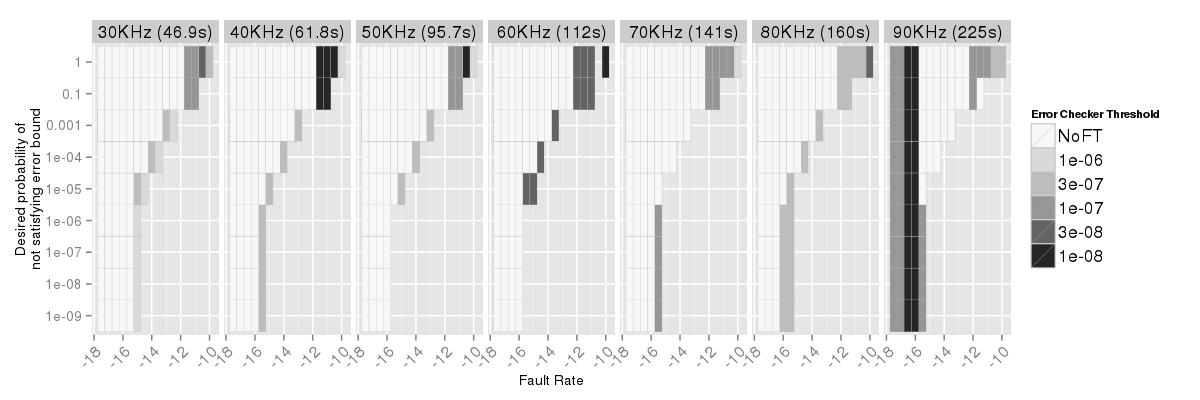
\includegraphics[width=7in]{figs/DRC_Serial_SuggestedConf.png}
\vspace{-10pt}
\caption{Suggested Resilience Technique for DRC Under the Serial Extrapolation Model Under Different Fault Rates}
\vspace{-10pt}
\label{fig:DRC_Serial_SuggestedConf}
\end{figure*}

\begin{figure}[ht!]
\centering
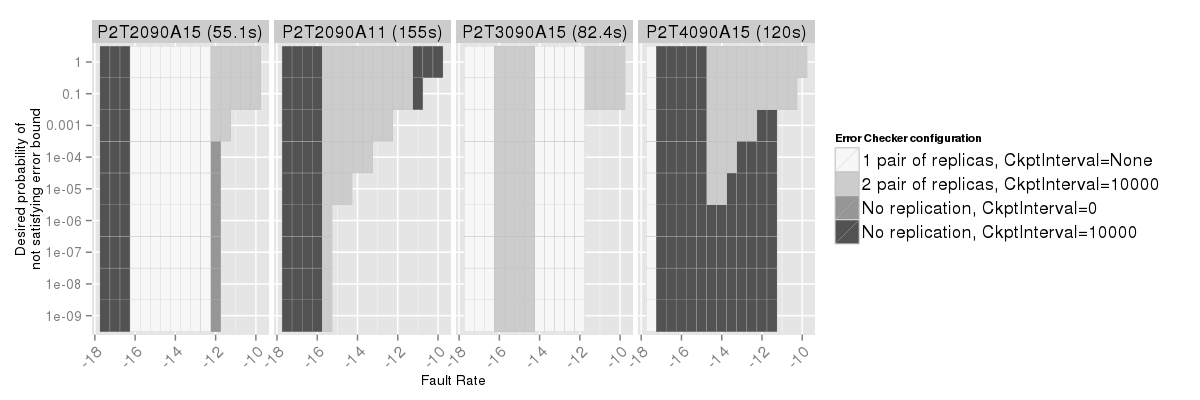
\includegraphics[width=3.4in]{figs/Hattrick_Parallel_SuggestedConf.png}
\vspace{-10pt}
\caption{Suggested Resilience Technique for Hattrick Under the Parallel Extrapolation Model Under Different Fault Rates}
\vspace{-10pt}
\label{fig:Hattrick_Parallel_SuggestedConf}
\end{figure}

\begin{figure}[ht!]
\centering
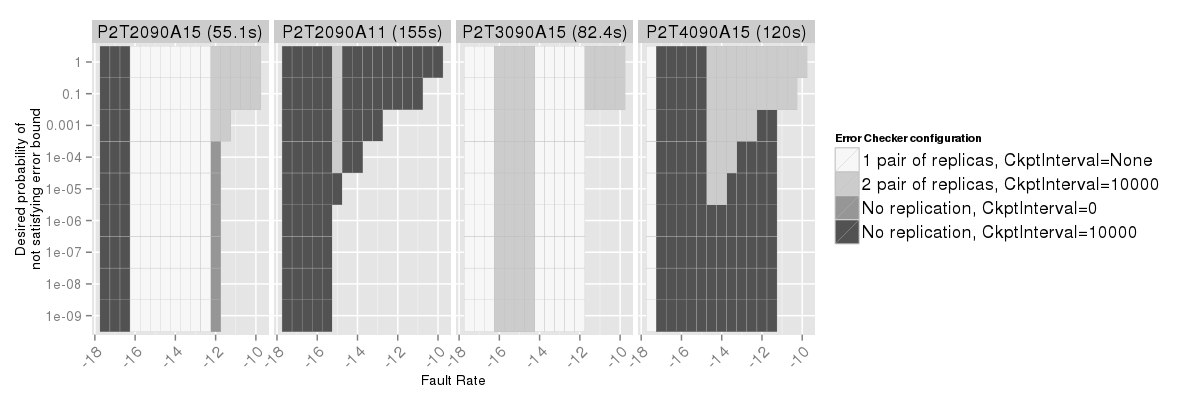
\includegraphics[width=3.4in]{figs/Hattrick_Serial_SuggestedConf.png}
\vspace{-10pt}
\caption{Suggested Resilience Technique for Hattrick Under the Serial Extrapolation Model Under Different Fault Rates}
\vspace{-10pt}
\label{fig:Hattrick_Serial_SuggestedConf}
\end{figure}



%\subsection{Overall Evaluation}
%\label{sec:eval:overall}

%%Experiment: Final graph that shows slowdown for each desired probability of perfect results.

\section{Summary}
\label{sec:summary}

In this paper we show that it is possible to effectively protect three real scientific applications from a wide range of faults by properly combining three different fault tolerant mechanisms:
Algorithmic error checks, replication of critical data structures and checkpoint-restart of individual routines.
We demonstrate that very significant improvements can be achieved in terms of reduction of performance slowdown and output numerical accuracy when scientific problems face error injection rates from $3 \cdot 10^{-11}$ and $3 \cdot 10^{-14}$ per processor cycle at 1Ghz, which are the expected rates in future high performance computing systems.
\sui{We have also demonstrated that the choice of the error checker threshold is important in achieveing a balance between result accuracy and overall performance. The choice is dependent on both the fault rate and the characteristics of the application.}
This work demonstrates that current scientific application can be safely executed on such systems if the programmers comprehensively combine a range of resilience techniques.

\bibliographystyle{abbrv}
\bibliography{bibs}

\end{document}
